\documentclass[12pt]{article}
\usepackage[utf8]{inputenc}
\usepackage{import}

\usepackage[OT1]{fontenc}
\usepackage[english]{babel}
\usepackage[toc,page]{appendix}
\usepackage{lipsum}
\usepackage{siunitx}
\usepackage{verbatim}
\usepackage{caption}
\usepackage{amsmath}
\usepackage{physics}

\usepackage{geometry}
\usepackage{bm} %Bold math symbols using \bm
\usepackage{authblk}
\usepackage{amssymb}
\usepackage{textcomp} %to get rid of warnings from gensymb
\usepackage{gensymb}
\usepackage{float}
\usepackage{hyperref} %\url{}
\usepackage{xurl}
\usepackage{braket} %dirac notation
\usepackage{diagbox}%\backslashbox{}{} in tabular
\usepackage{stackengine} %stacking (for making new commands)
\usepackage{scalerel} %scaling (for making new commands)

%Images
\usepackage{titlepic}%title pic
\usepackage{wrapfig}
\usepackage{graphicx}%to manage images
\usepackage{grffile}%to don't print the file name
\usepackage{subfig}%two pictures in one \subfloat[name]{}
\usepackage{pdfpages} %helsida \incudepdf{}


\makeatletter
\patchcmd{\@maketitle}{\LARGE \@title}{\fontsize{16}{19.2}\selectfont\@title}{}{}
\makeatother

\renewcommand\Authfont{\fontsize{12}{14.4}\selectfont}
\renewcommand\Affilfont{\fontsize{9}{10.8}\itshape}

\newgeometry{left=2.5cm, bottom=0.6cm, right=2.5cm, top=3.5cm}

\title{MNXB01: Investigation of SMHI weather data}
\author{Eleftheria Kosta, Felipe Abedrapo, Simon Tropp, Tanvir Sayed}
\affil[1]{The Faculty of Science, Department of Physics, Lund University}


\titlepic{
\vspace{1cm}
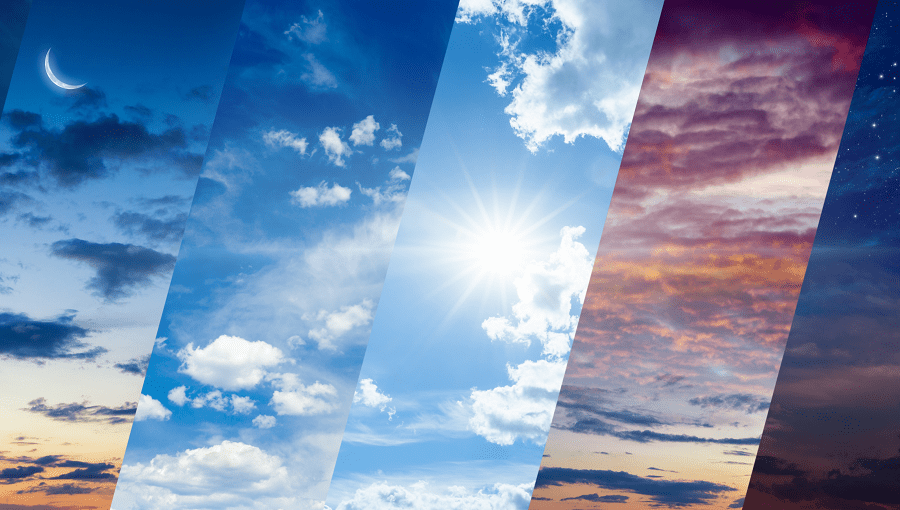
\includegraphics[width=0.9\linewidth]{Images/titlepage.png}}
\renewcommand{\baselinestretch}{1.5}


\begin{document}
    \clearpage
    \maketitle
    \thispagestyle{empty}
    \vspace*{\fill}
    \begin{flushleft}
        \textbf{Course responsible:} Oxana Smirnova\\
    \end{flushleft}
    
    \begin{figure}[H]
        \centering
        
\includegraphics[scale=1.1]{Images/Lund logo science1.png}
    \end{figure}
    
    \newpage
    \newgeometry{left=2.5cm, bottom=2.5cm, right=2.5cm, top=2.5cm}

\section{Introduction}
The goal of this project was to analyse and investigate weather data from the Swedish Meteorological and Hydrological Institute (SMHI). The datasets considered in this project contain a number of temperature measurements for each day during the past $\sim100$ years. Using the temperature data, it is possible to investigate multiple theories and research within meteorology. 
\newline
In this project, the daily temperatures on a specific day (throughout the years) is investigated and plotted in a histogram. Through the histogram it will be possible to observe the behavior of the daily temperatures, and from its distribution it could be concluded whether it has a standard Gaussian behavior. Alternatively, if the behavior and trend of the daily temperatures tend to have a more smeared out peak, or a second peak for higher temperatures, possible connections can be drawn to global warming. The project also investigates the correlation between the maximum and minimum temperatures of each year. Finally, investigation of the season length is considered. Specifically, by counting the days passed between every year's maximum temperature, it is possible to conclude whether there always are about 365 days between each midst of the summer, or if there is a certain trend of the seasonal year getting longer/shorter.



\newpage
\section{Method}
\subsection{Code Structure and External Libraries}
The code is structured in a way such that the results are produced in a file called project.cpp. This main function (called just 'project' in this case) makes use of the headers 'parse\_csv.h' and 'tempTrender.h' which are contained in the /include directory. The tempTrender header contains a class called tempTrender where an object is initialized by passing in a filename containing weather data as a parameter. The member functions tempOnDay, max/minOverTime, and avgDailyTempOverTime act on the object by parsing through the csv, extracting the data, processing it, and then plotting it using ROOT libraries. To parse through the csv Ben Strasser's Fast C++ CSV Parser (\url{https://github.com/ben-strasser/fast-cpp-csv-parser}) was used by cloning the github repository into an directory called ./external/include. With this library one could quickly go through every line of the csv file and extract information depending on the Result one is looking to create. 

\subsection{Cleaning the dataset files for use}
To perform a proper and convenient analysis of the weather data, the datasets from the SMHI first needed to be 'cleaned' and stored as a csv file that could be easily read by the csv file parsing library that was used. For that purpose, the two bash scripts 'ProduceCleanDatasets.sh' and 'smhicleaner.sh' were written. The smhicleaner.sh script uses bash commands to look for the city of interest in the dataset folder containing files for the different cities. If the file for the city is found, unnecessary strings and lines are removed keeping only the rawdata of the date, time, temperature, and quality (along with these as column headers). The data in the rows are changed to be separated by commas so it is now in csv format. The ProduceCleanDatasets.sh script , which should be run from the base folder 'Final\_Project\_TeamB', takes the city name as a input parameter and uses the smhicleaner.sh script to do the cleaning of the dataset and put the clean datafile with the name Clean'City' in the code/ClnData folder where it is to be accessed and used by the other C++/Root coded functions.     

\subsection{Histogram of temperatures on a specific day through time}
In this portion of the project, a month and a day is given as input by the user (along with the filepath containing the weather data of the city in question) and the function tempOnDay parses through the CSV, extracts the temperatures for the given day, plots it as a histogram and then performs a Gaussian fit on it. The algorithm for extracting the data starts by turning the inputted month and day into a string that can be compared with the dates provided in the CSV. Then, the downloaded CSV parser is used to read the file line by line within a specific year and then pushes the temperature value for the specific day into a vector. This is done for every year available in the data meaning that the size of the final vector is that of the amount of years available. Finally, this vector is used as the data source for a histogram plotting function.


\subsection{Investigating the max and min temperatures through the years}
The algorithm used for the function \texttt{maxTempOverTime()} is that the CSV parser is used to retrieve a list with all the years available. Then, for each year in the list, the code stores the daily temperatures in a vector and once the year is over, it finds the maximum temperature and pushes it to another vector called \texttt{max\_temp\_vector}. This vector is then used to create a plot of the maximum temperature over time and to look for trends. The \texttt{minTempOvertime()} function works the same way except that it pushes the minimum temperature rather than the max. 


\subsection{Investigating the daily mean temperature}
To find the daily mean temperature over time, we first parse through the file and extract every date possible and store it in a vector called \texttt{all\_datums}. For efficiencies' sake it was important that these are ordered cronologically. Then, for each date in \texttt{all\_datums}, the parser goes through the lines of the files and stores the temperature in a vector if the dates correspond to each other. Once they stop corresponding the temperatures are averaged and pushed to a vector called \texttt{dailyTempOverTime()}.
\newline
\newline
To find the days at which the max average daily temperatures occur per year, the function \texttt{Day\_MaxAvgTemp()} was written. This function parses through the dataset file for a city and for each year, it finds the daily average temperatures and stores them in a vector. A vector of the dates in the year is also stored. The maximum temperature in this vector for the current year is recorded and the index of the maximum temperature in the vector is located with another function \texttt{getIndexOfTemp} that was written. The index (i.e) reference in the date vector for the year corresponds to the day of this max temperature, and is stored in another vector \texttt{Day\_MaxAvgTemp\_Year}. As all the years are looped through the file, all the dates for the yearly maximum temperatures are stored.
\newline
\newline
Next, to find the distance (i.e days) between the yearly maximum temperatures, the dates returned by the \texttt{Day\_MaxAvgTemp()} function is compared to all the dates in the datafile, with a day counter that keeps track of the day number starting from the first day of the file  to the last. When the dates match, the day counter is stored as the last element in a \texttt{DayNoList} vector. The difference between this last element in \texttt{DayNoList} vector and the next day counter (when dates match again) is found to find the distance between the yearly maximum temperatures and stored in the \texttt{DiffList} vector. 

\newpage
\section{Results \& Interpretations}
\subsection{Temperatures on a day}
The member function \texttt{tempOnDay()} (corresponding to the \texttt{class tempTrender}) creates a histogram with the temperatures recorded for a specific day given as an input by the user. It tries to fit the histogram with a Gaussian distribution as well. An example for this is shown in Figure \ref{fig:LundTeml}. In the figures, one can see the change in mean temperature and spread through the different months. This indicates how the temperature distribution changes with the seasons. During summer, around June-September the temperature is much higher compared to winter, around December-March. 
\begin{figure}[H]
    \centering
    \subfloat[March 6th]{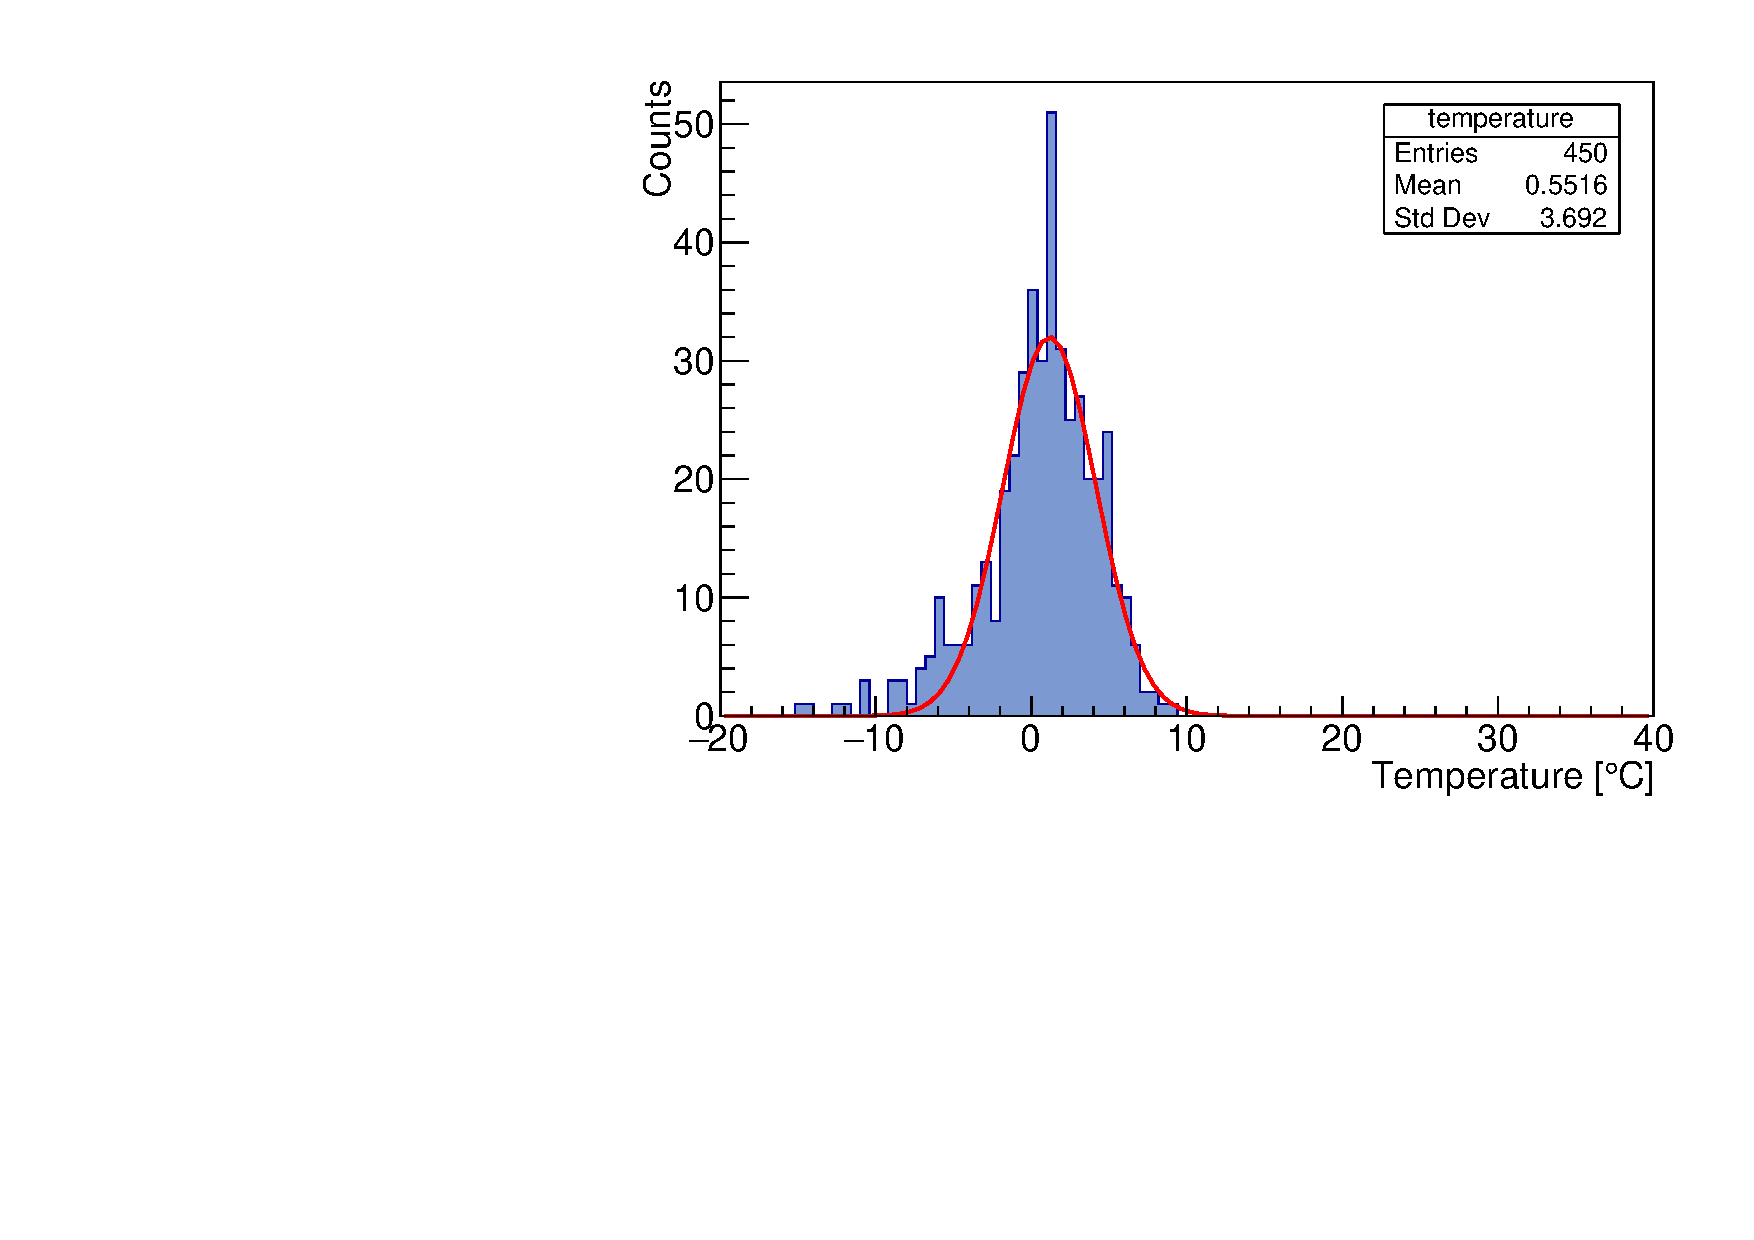
\includegraphics[width=0.49\linewidth]{Images/Lund3-3.pdf}}
    \subfloat[June 6th]{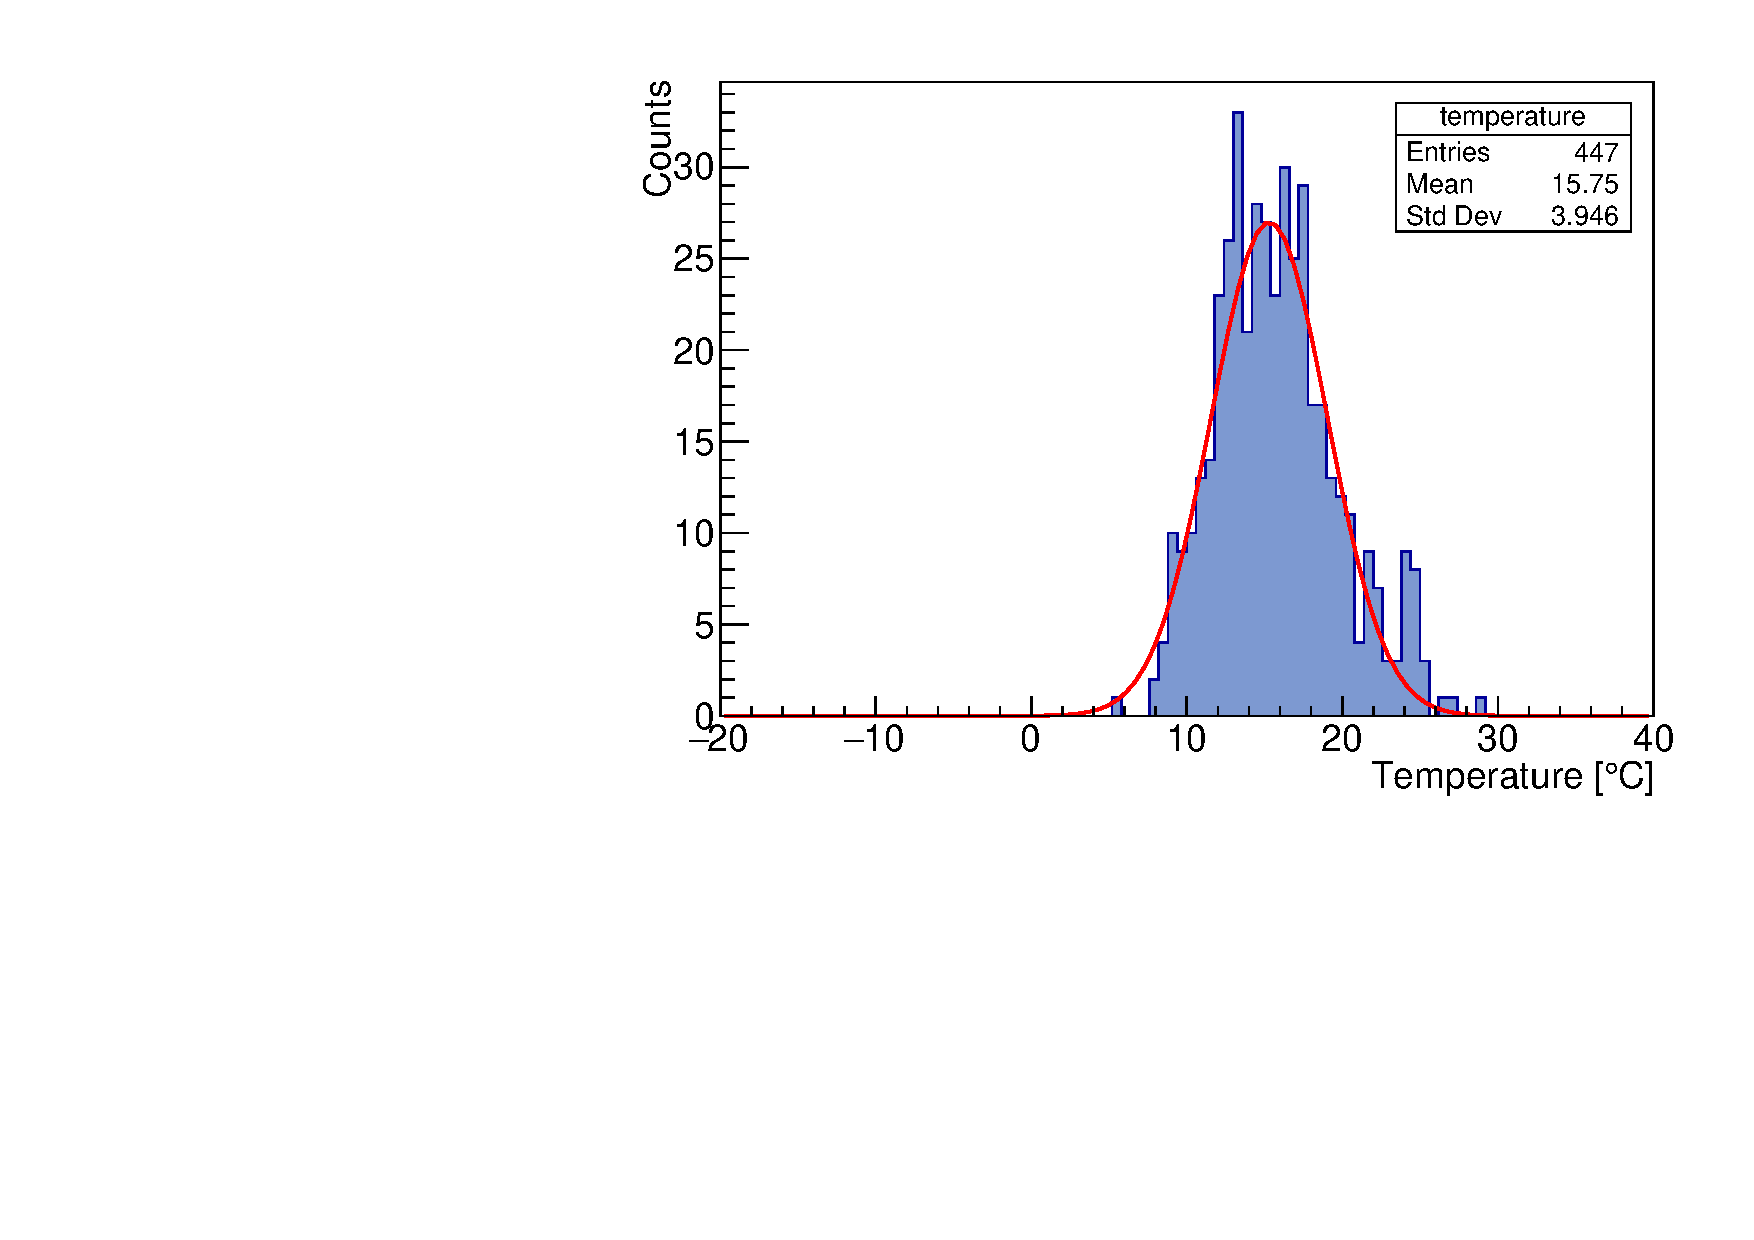
\includegraphics[width=0.49\linewidth]{Images/Lund6-6.pdf}}
    \quad
    \subfloat[September 6th]{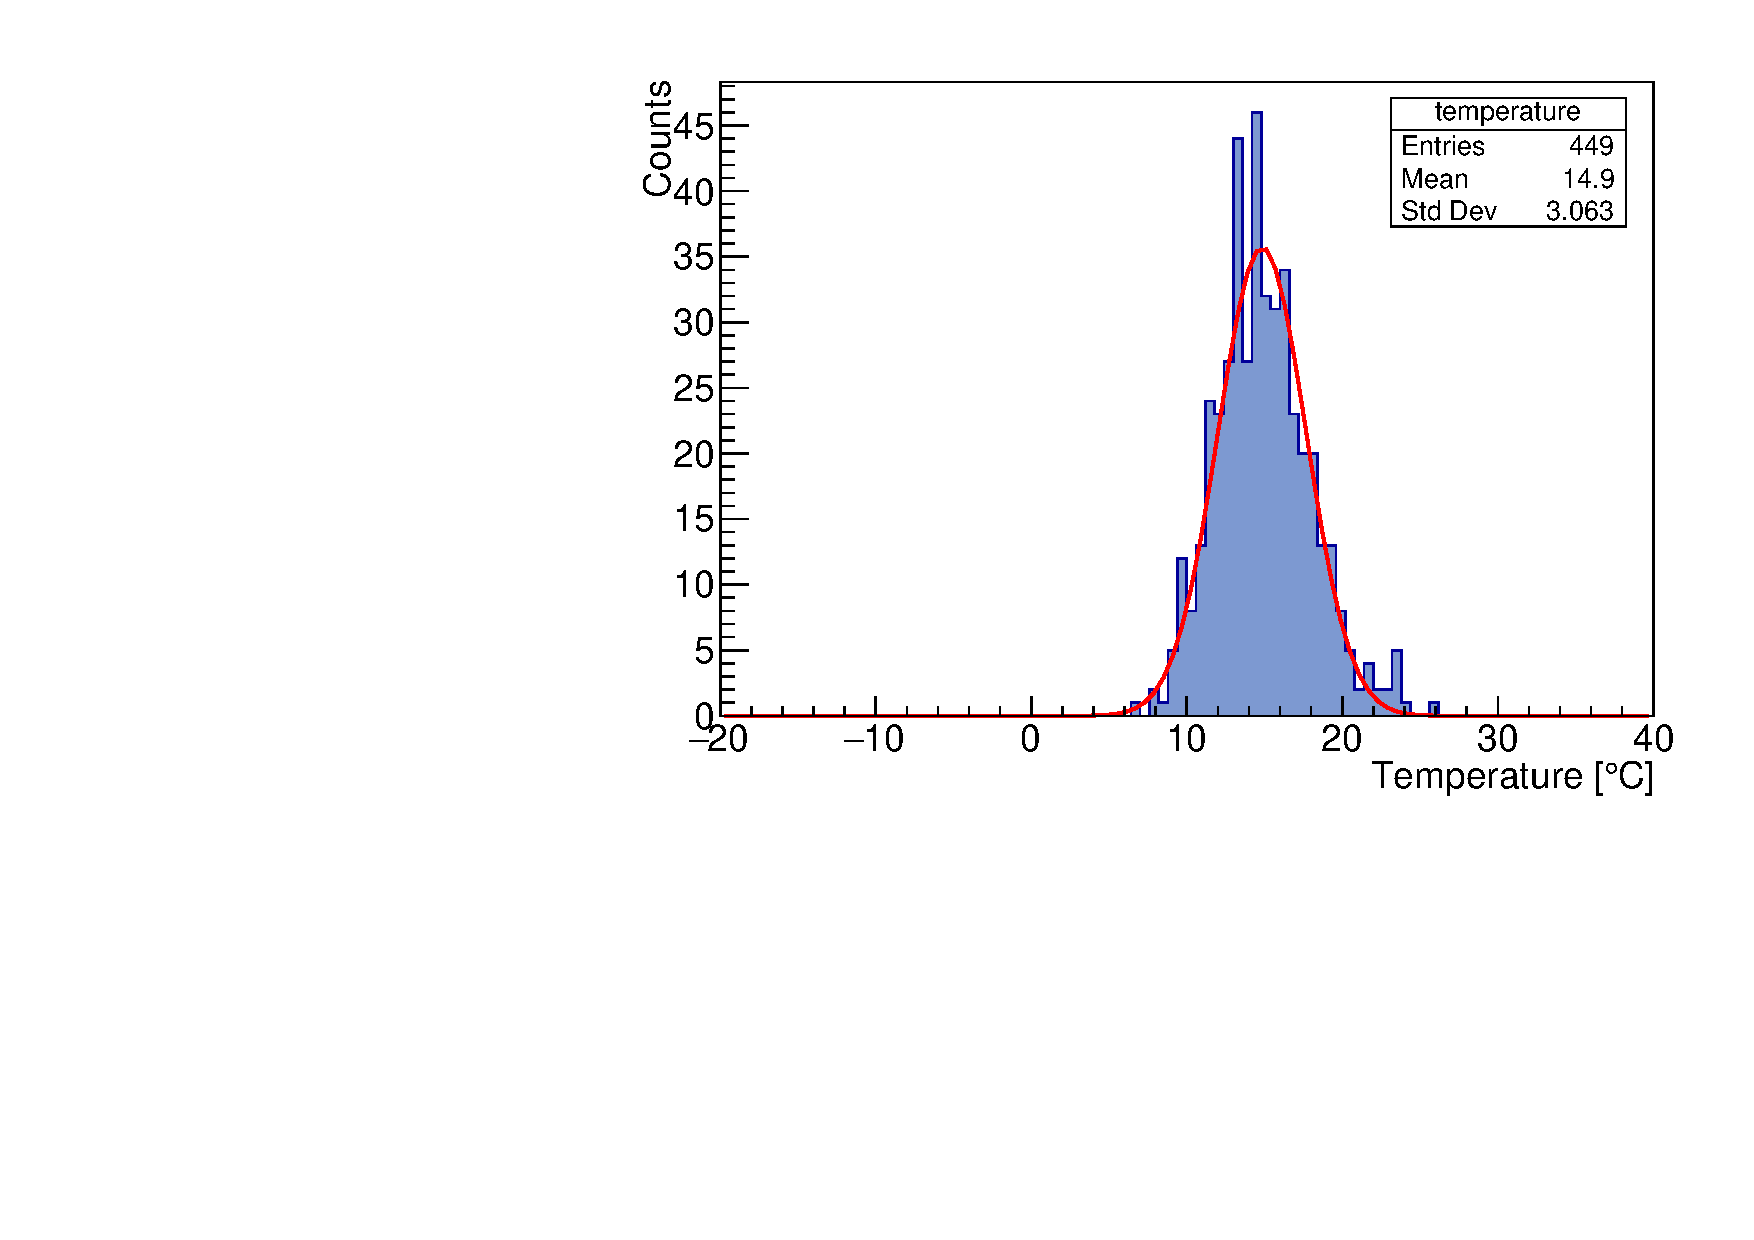
\includegraphics[width=0.49\linewidth]{Images/Lund9-6.pdf}}
    \subfloat[December 6th]{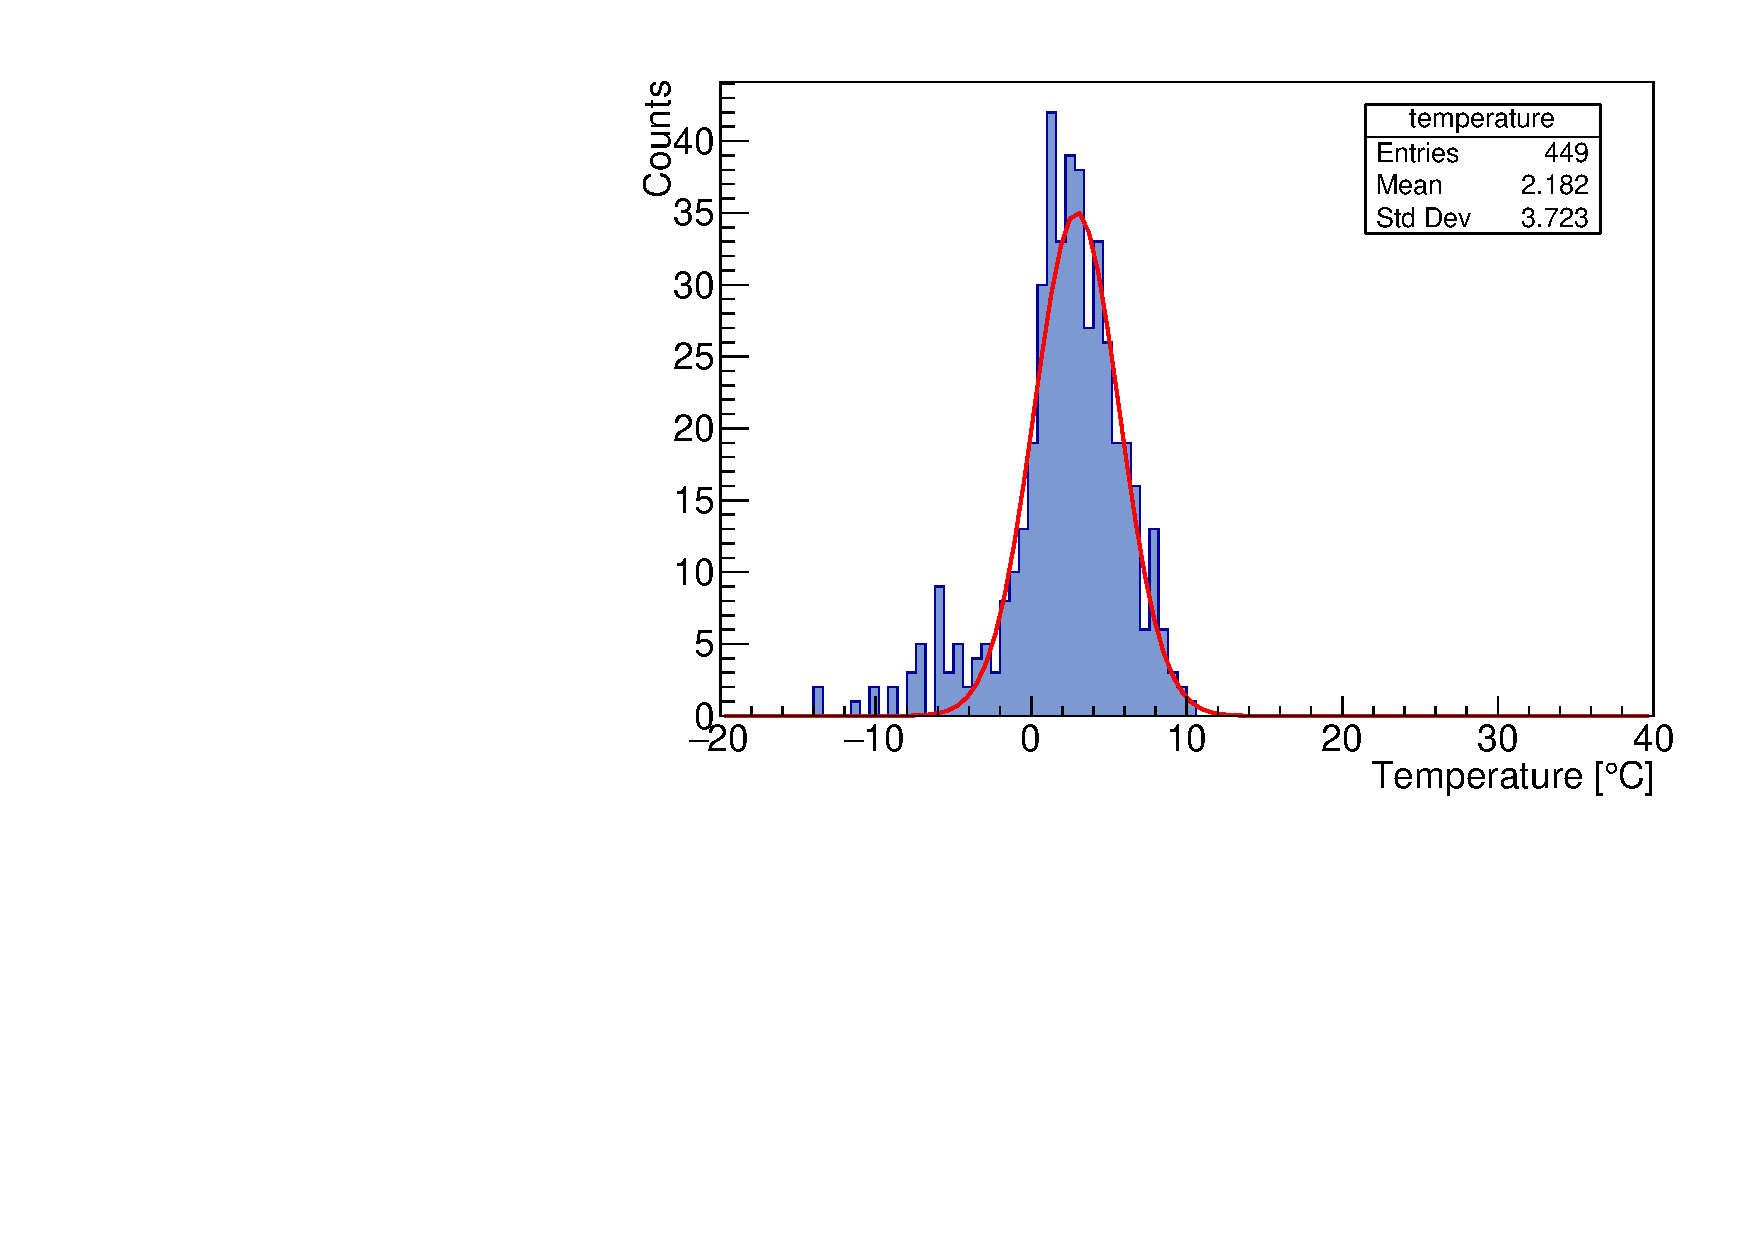
\includegraphics[width=0.49\linewidth]{Images/Lund12-6.pdf}}
    \caption{Temperatures in Lund}
    \label{fig:LundTeml}
\end{figure}

\noindent Since the distribution seemed normal, it was possible to use the ROOT fitting functions to do a gaussian fit and know the average temperatures as well as their standard deviations. The temperatures change over the year as expected and they have standard deviations from the average by 3-4 degrees. This is different to the case in cities which are located in the northernmost part of Sweden such as Luleå where the distribution is not quite normal. In Figure \ref{LuleåTemp}, we can see an almost exponential distribution and therefore the Gaussian fit does not provide any meanful information in this case. Although, the number of data points of temperatures measured might not have been enough to show the actual distribution which might be a Gaussian (as one can see the entries for Luleå were less than half than for Lund).



\begin{figure}[H]
    \centering
    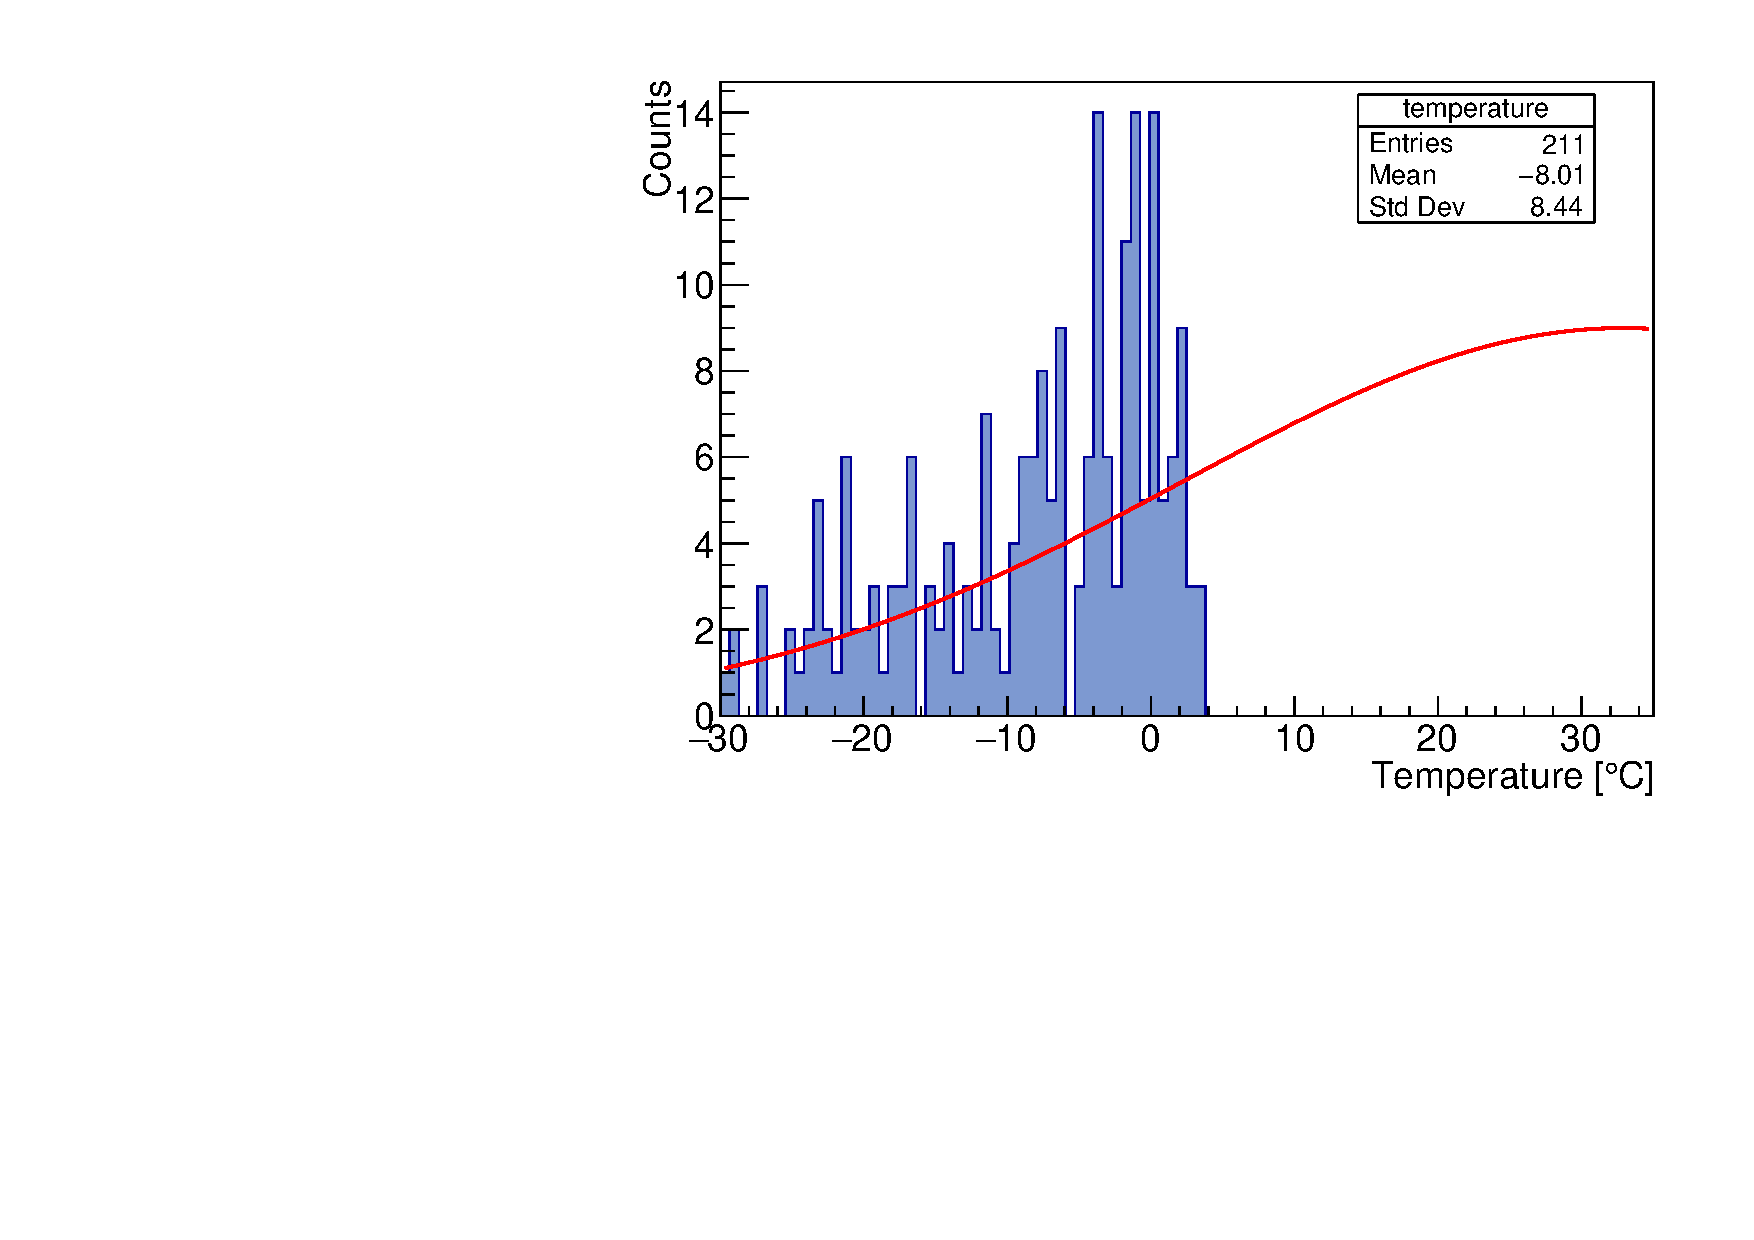
\includegraphics[scale=0.6]{Images/lulea_histogram.pdf}
    \caption{Histogram of the Temperature in Luleå on December 15}
    \label{LuleåTemp}
\end{figure}
One could also compare the temperatures for different cities for the same day as in Fig \ref{fig:Cities}. Although, the mean temperature is not that different for the different cities, it is noticed that as one goes more North the temperature drops slightly.

\begin{figure}[H]
    \centering
    \subfloat[Falsterbo]{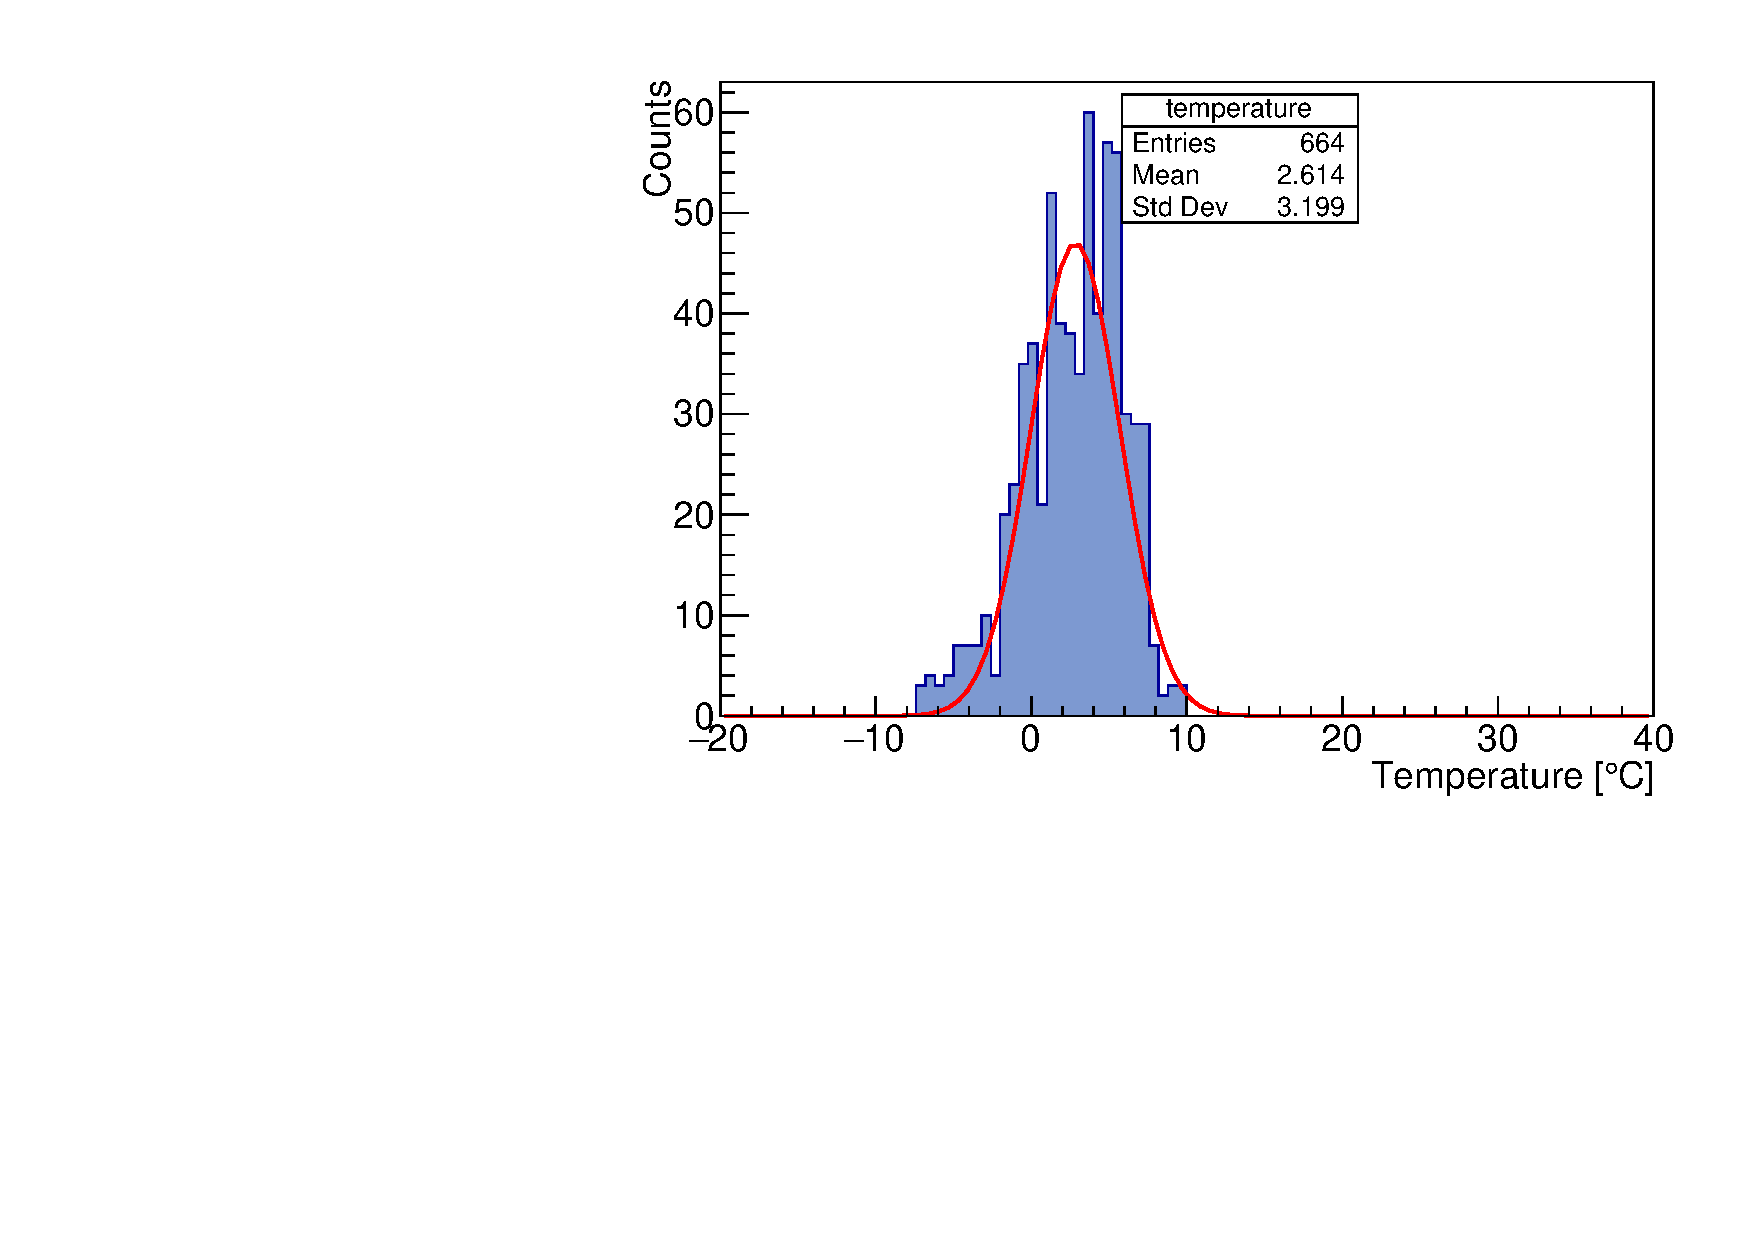
\includegraphics[width=0.49\linewidth]{Images/Task1Images/Falsterbo1215.pdf}}
    \subfloat[Borås]{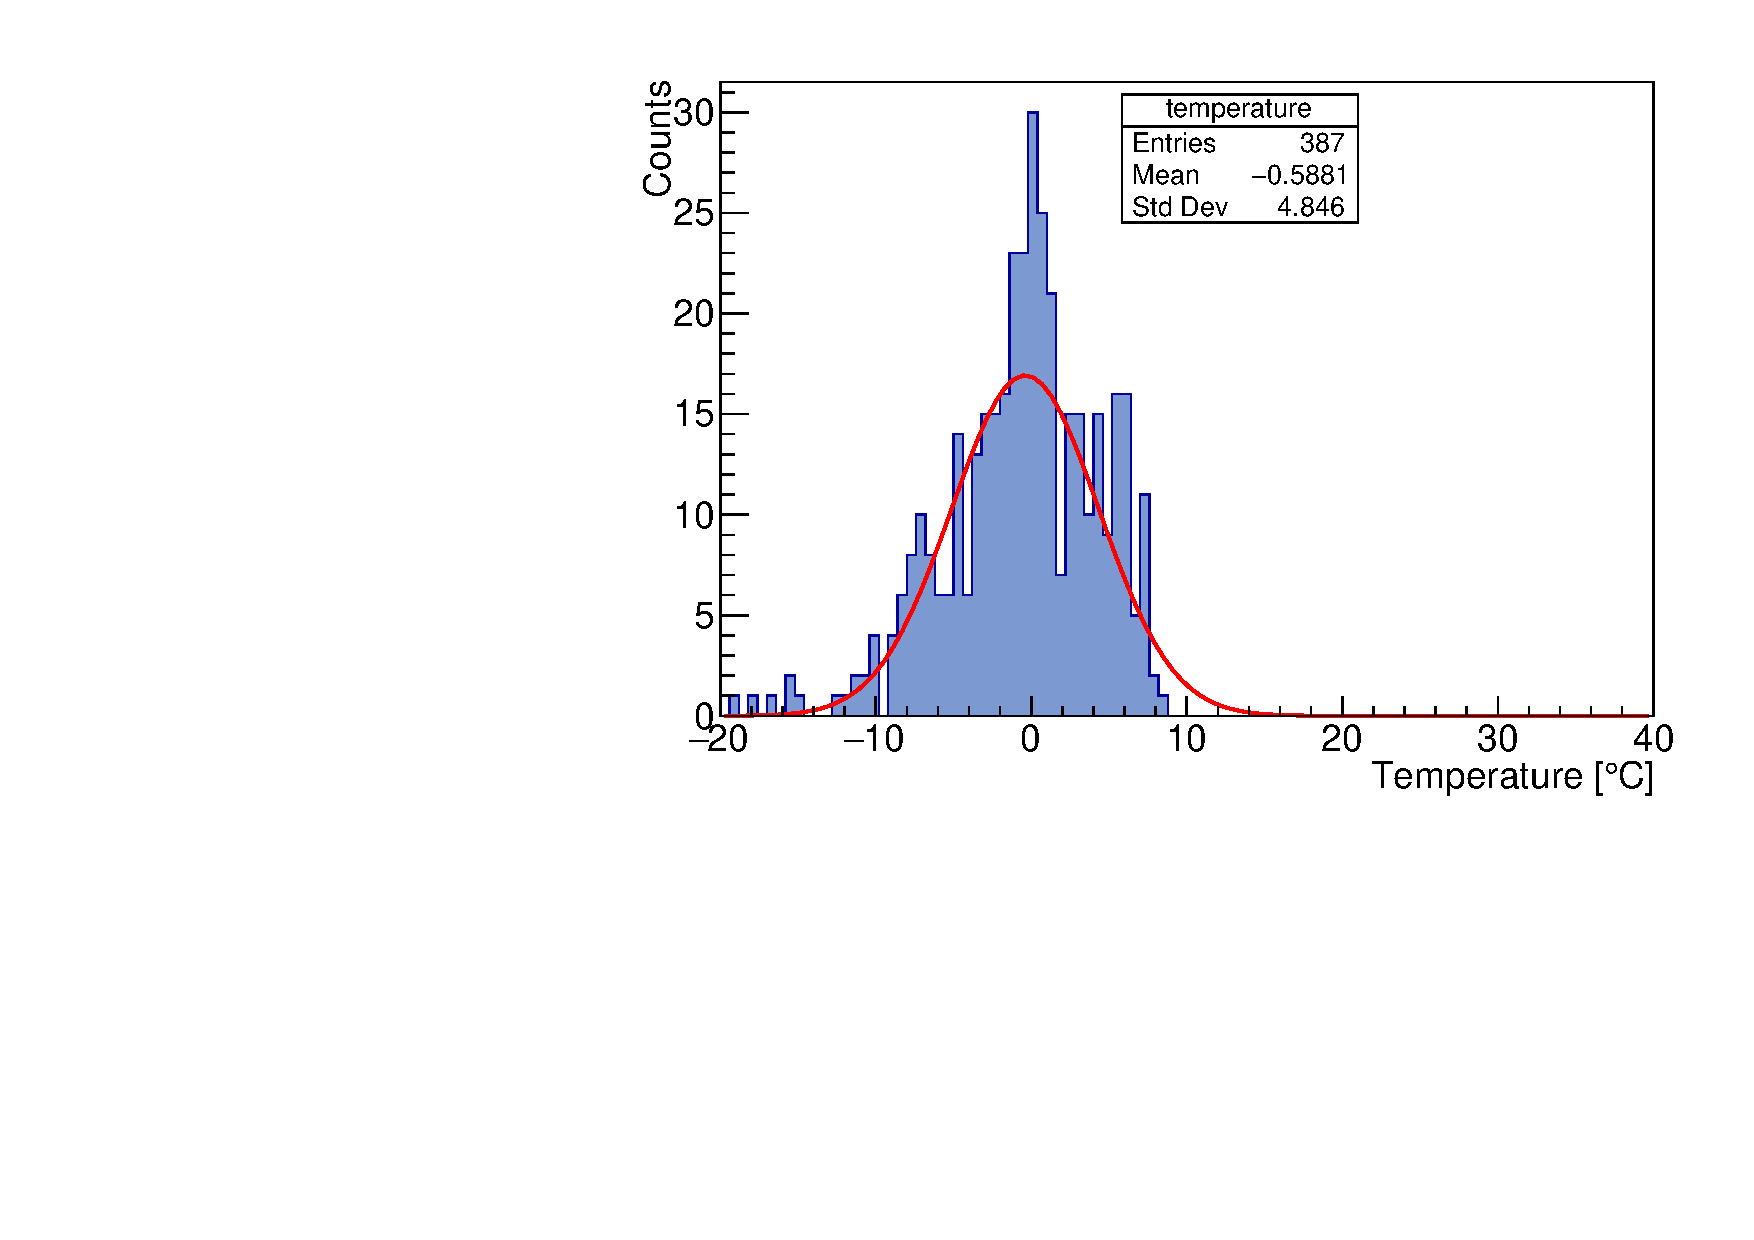
\includegraphics[width=0.49\linewidth]{Images/Task1Images/Boras.pdf}}
    \quad
    \subfloat[Karlstad]{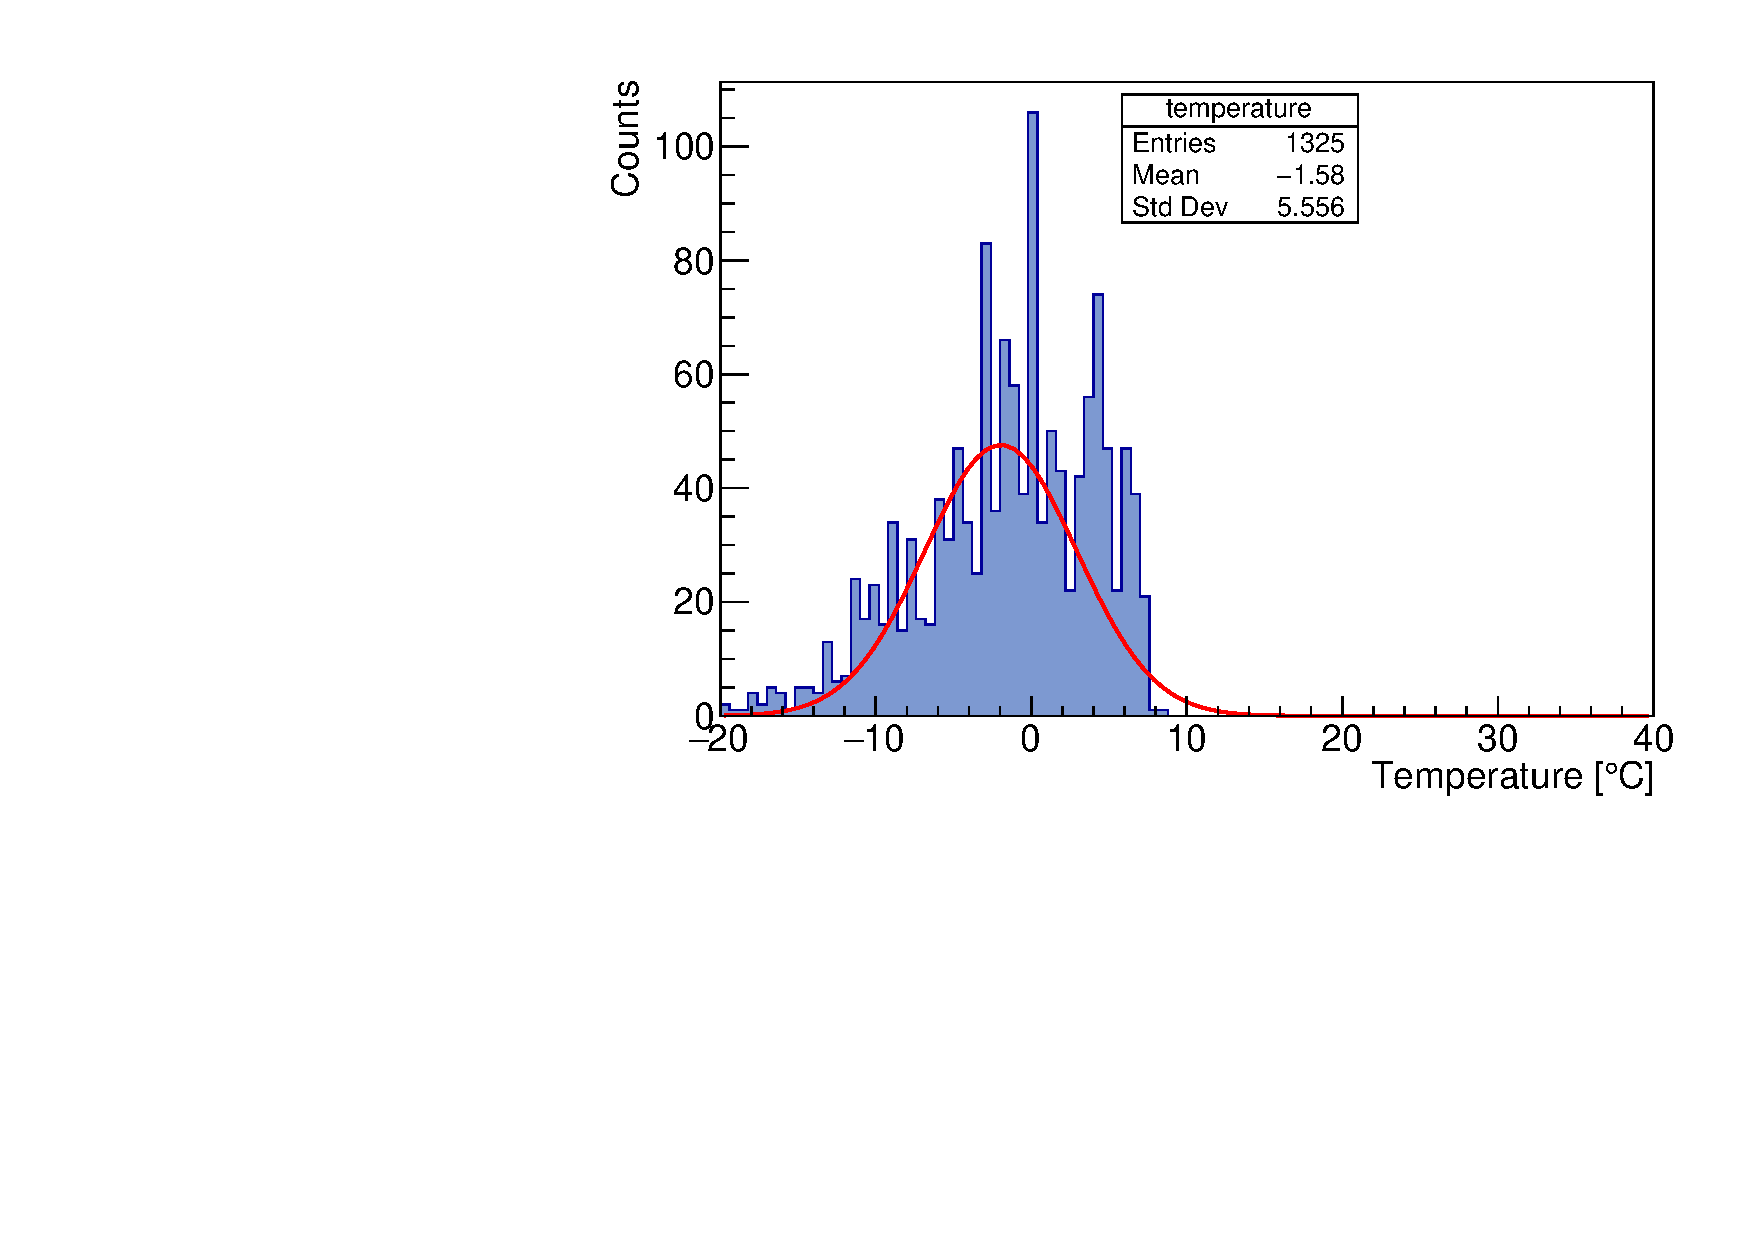
\includegraphics[width=0.49\linewidth]{Images/Task1Images/Karlstad1215.pdf}}
    \subfloat[Falun]{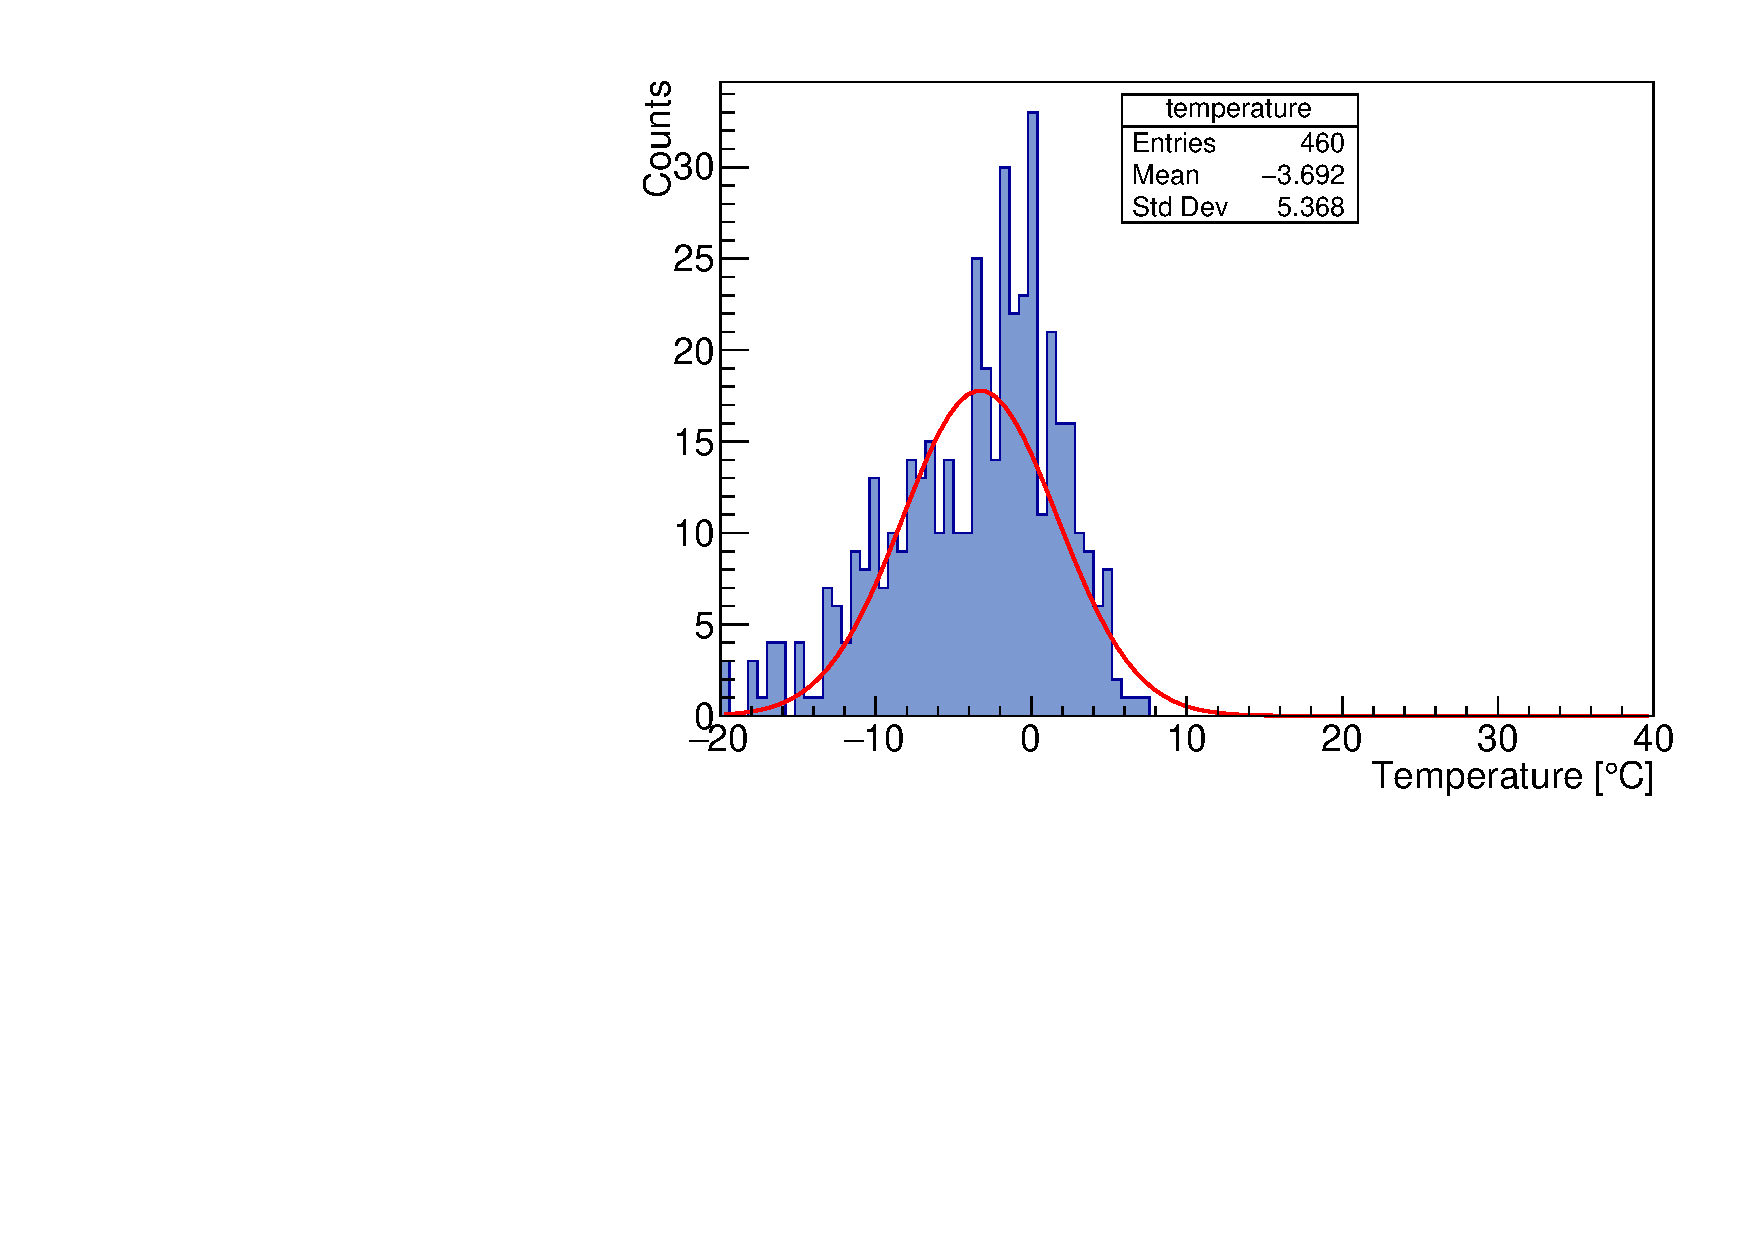
\includegraphics[width=0.49\linewidth]{Images/Task1Images/Falun1215.pdf}}
    \caption{Temperatures in different cities on December 15.}
    \label{fig:Cities}
\end{figure}

\newpage
\subsection{Yearly max and min temperatures}
In this part, the maximum and minimum temperatures for a given city were found and plotted over time. In figure \ref{fig:MinMaxTemp}, the maximum and minimum temperatures are given for 4 cities, Falsterbo, Lund, Borås and Umeå.
\begin{figure}[H]
    \centering
    \subfloat[Falsterbo]{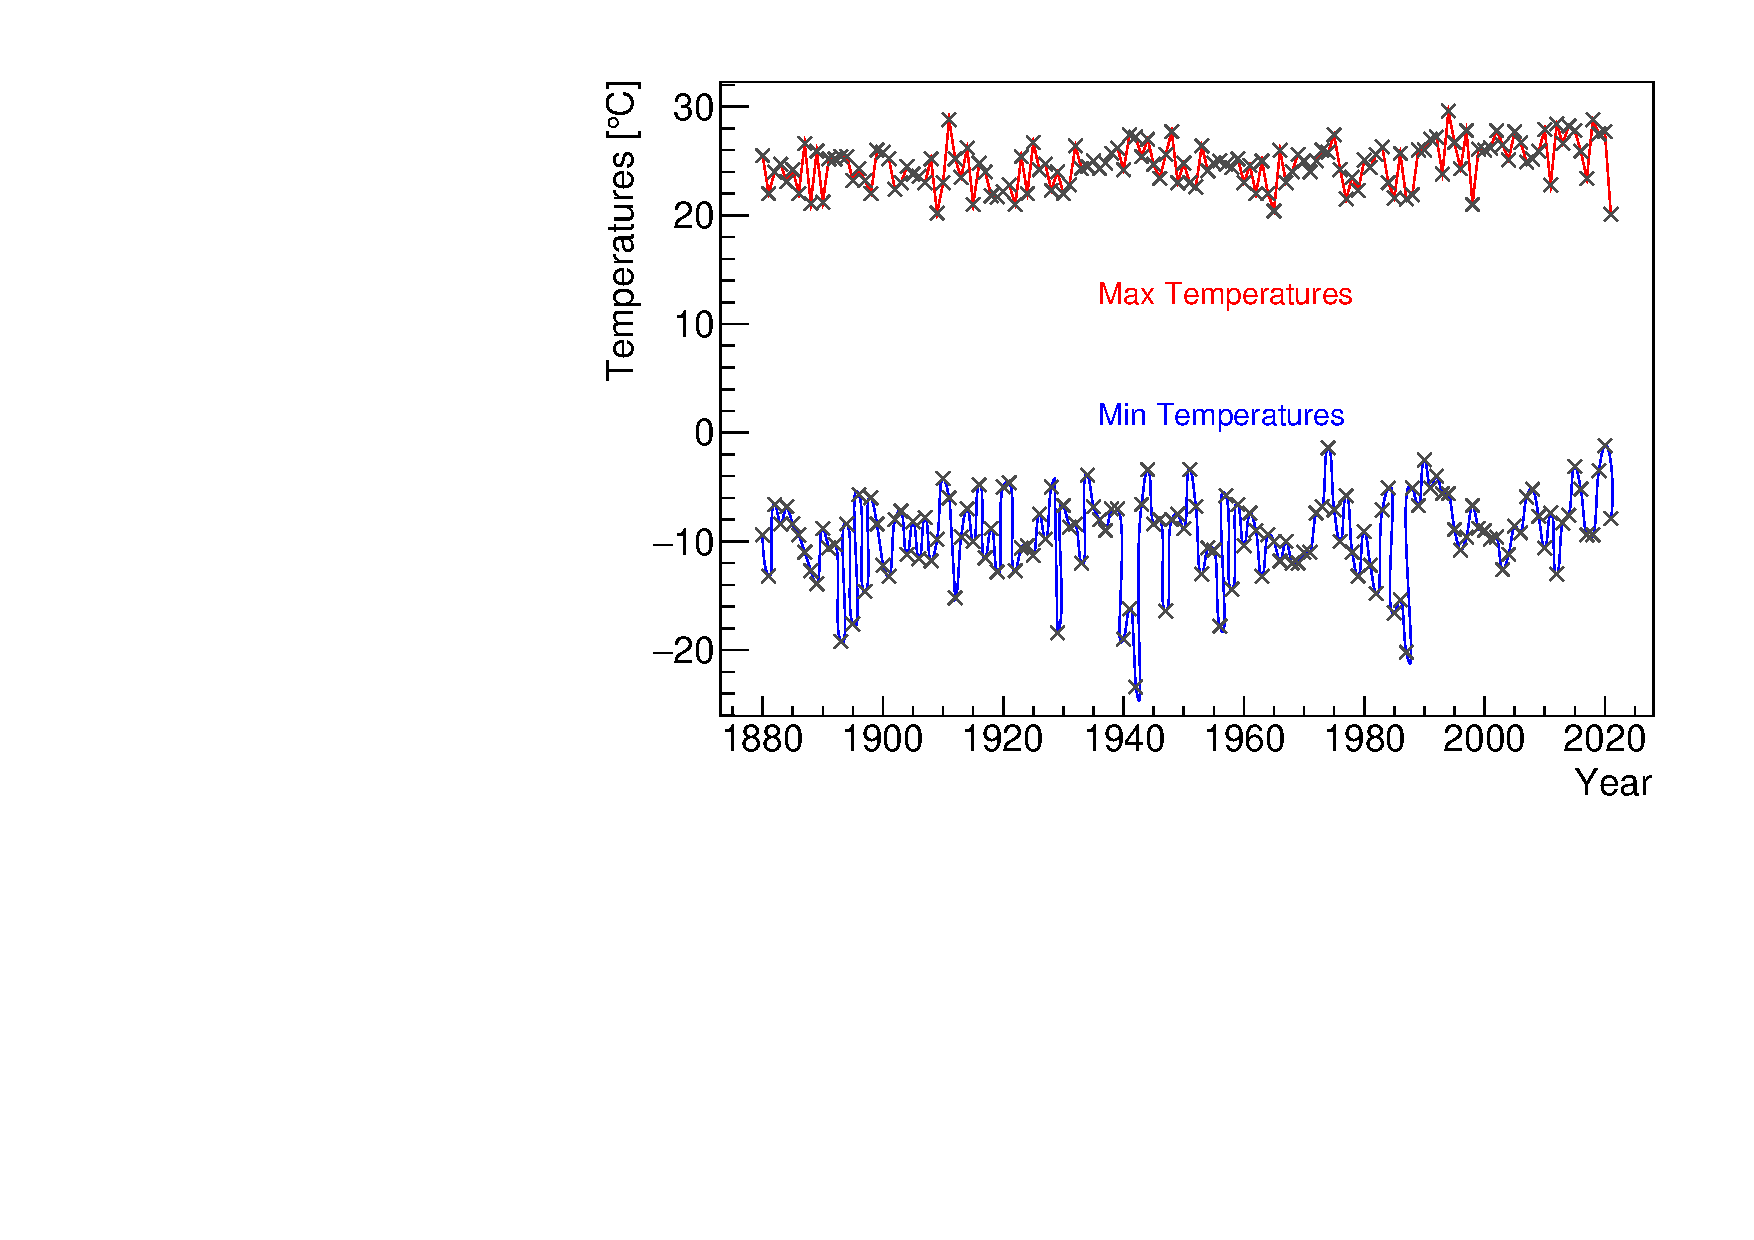
\includegraphics[width=0.5\linewidth]{Images/minmax_falsterbo.pdf}}
    \subfloat[Lund]{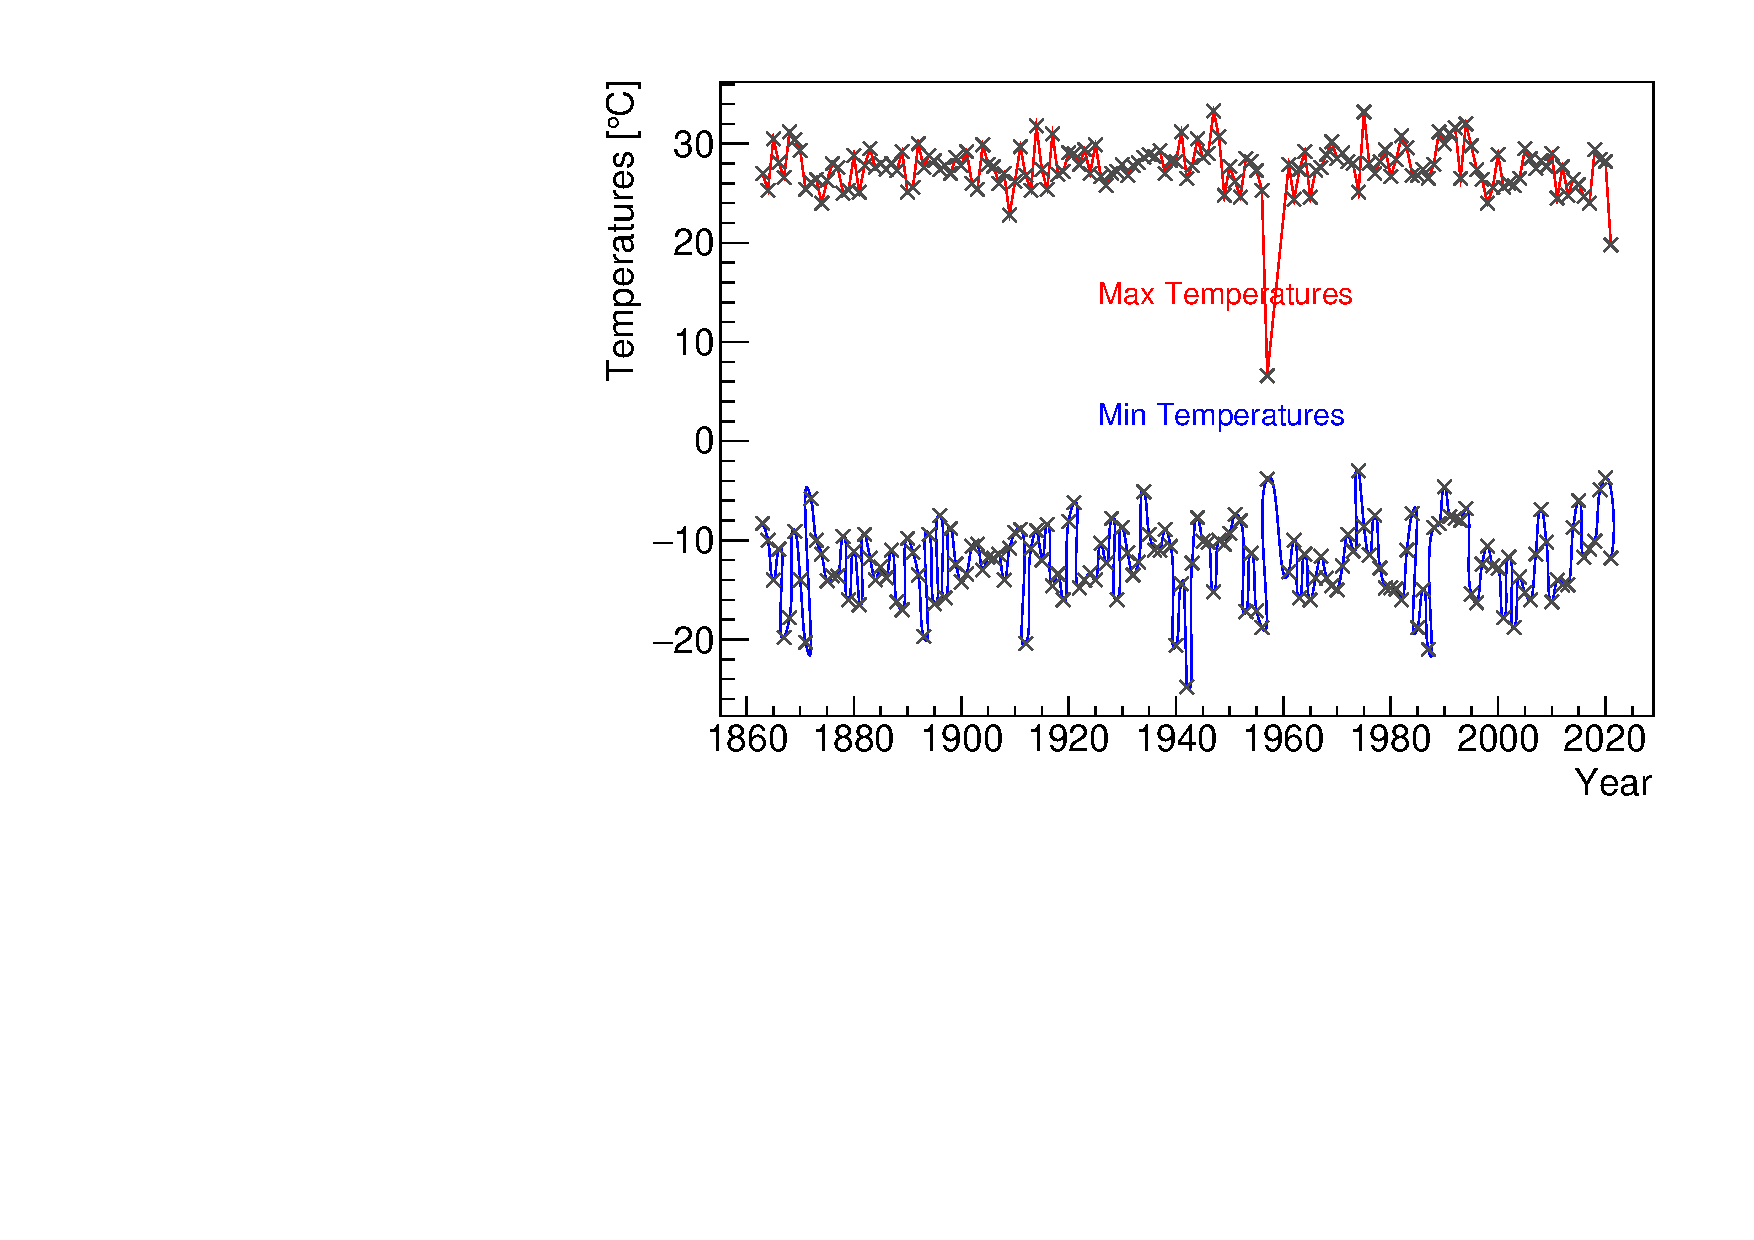
\includegraphics[width=0.5\linewidth]{Images/minmax_lund.pdf}}
    \quad
     \subfloat[Borås]{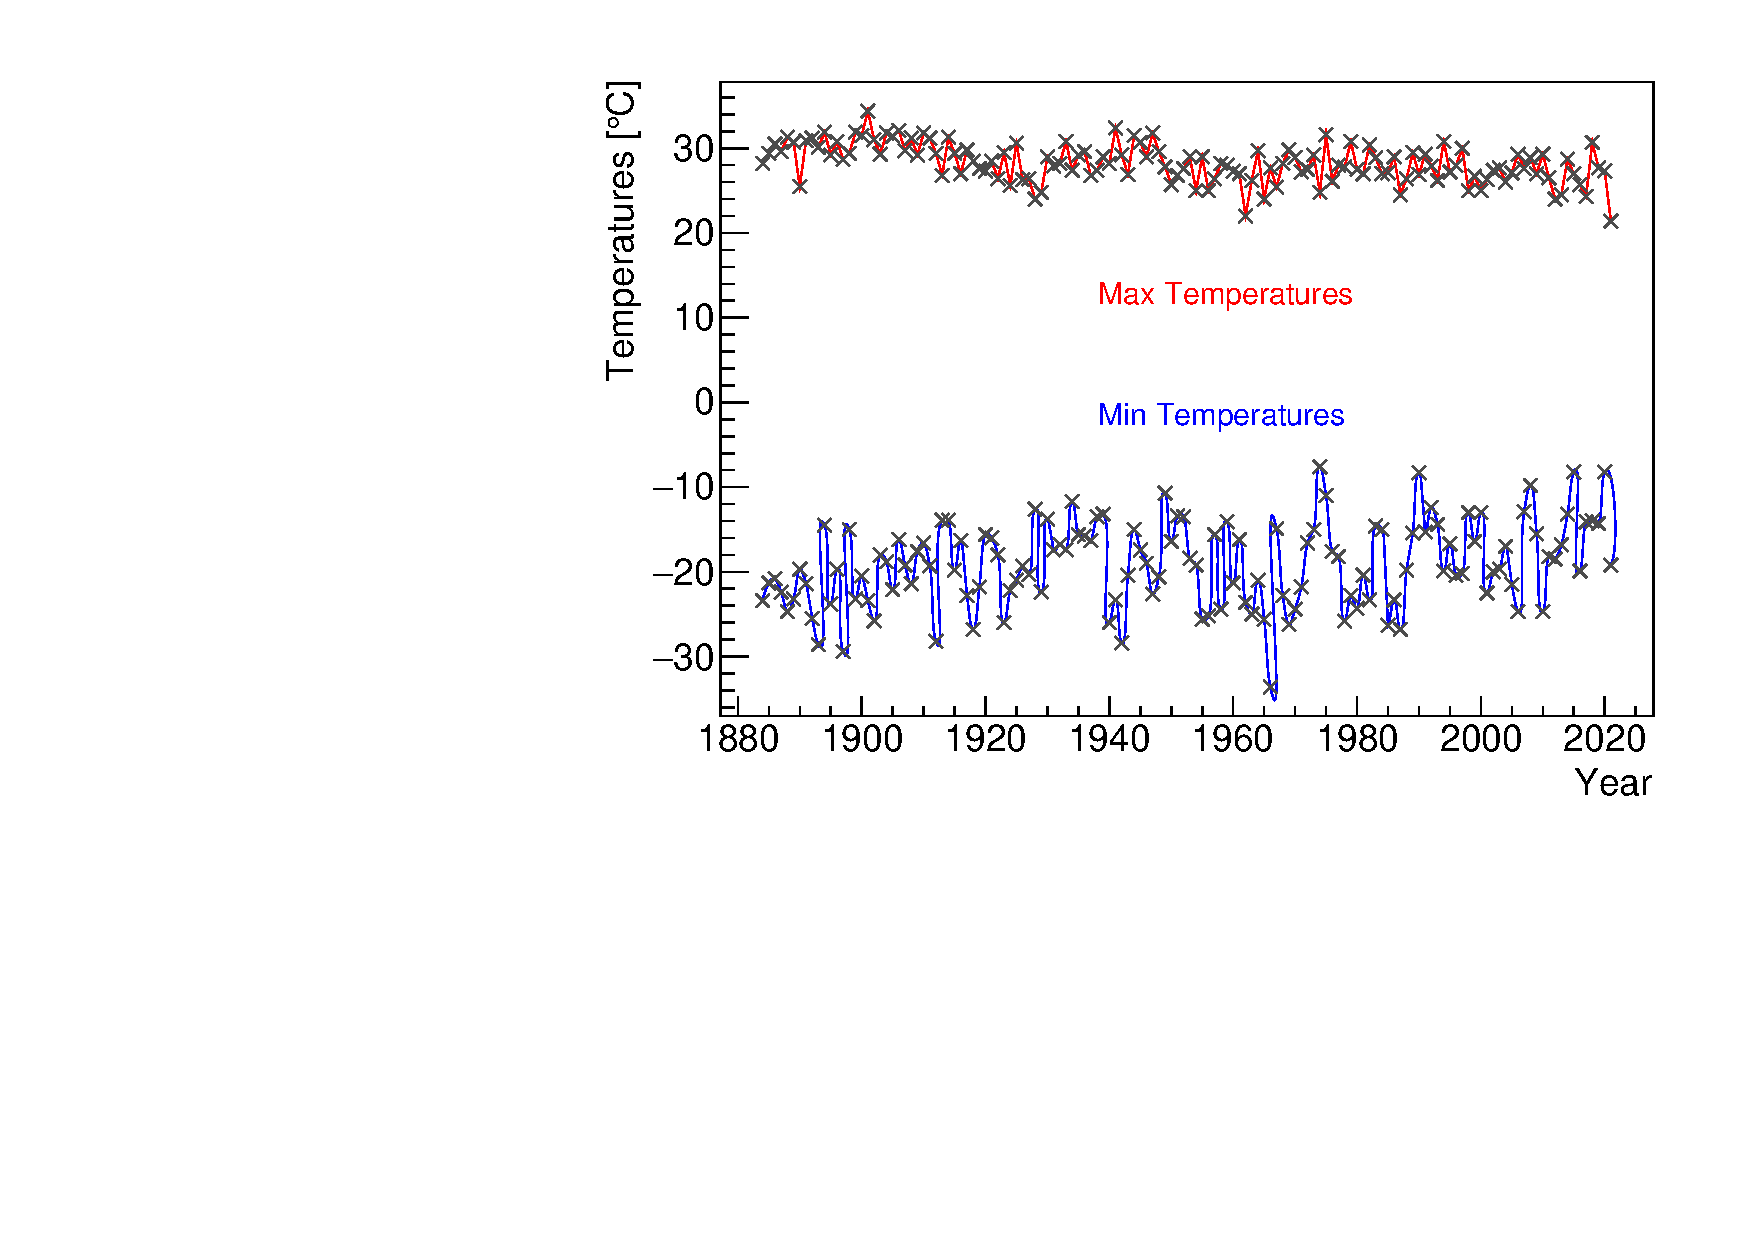
\includegraphics[width=0.5\linewidth]{Images/minmax_Boras.pdf}}
     \subfloat[Umeå]{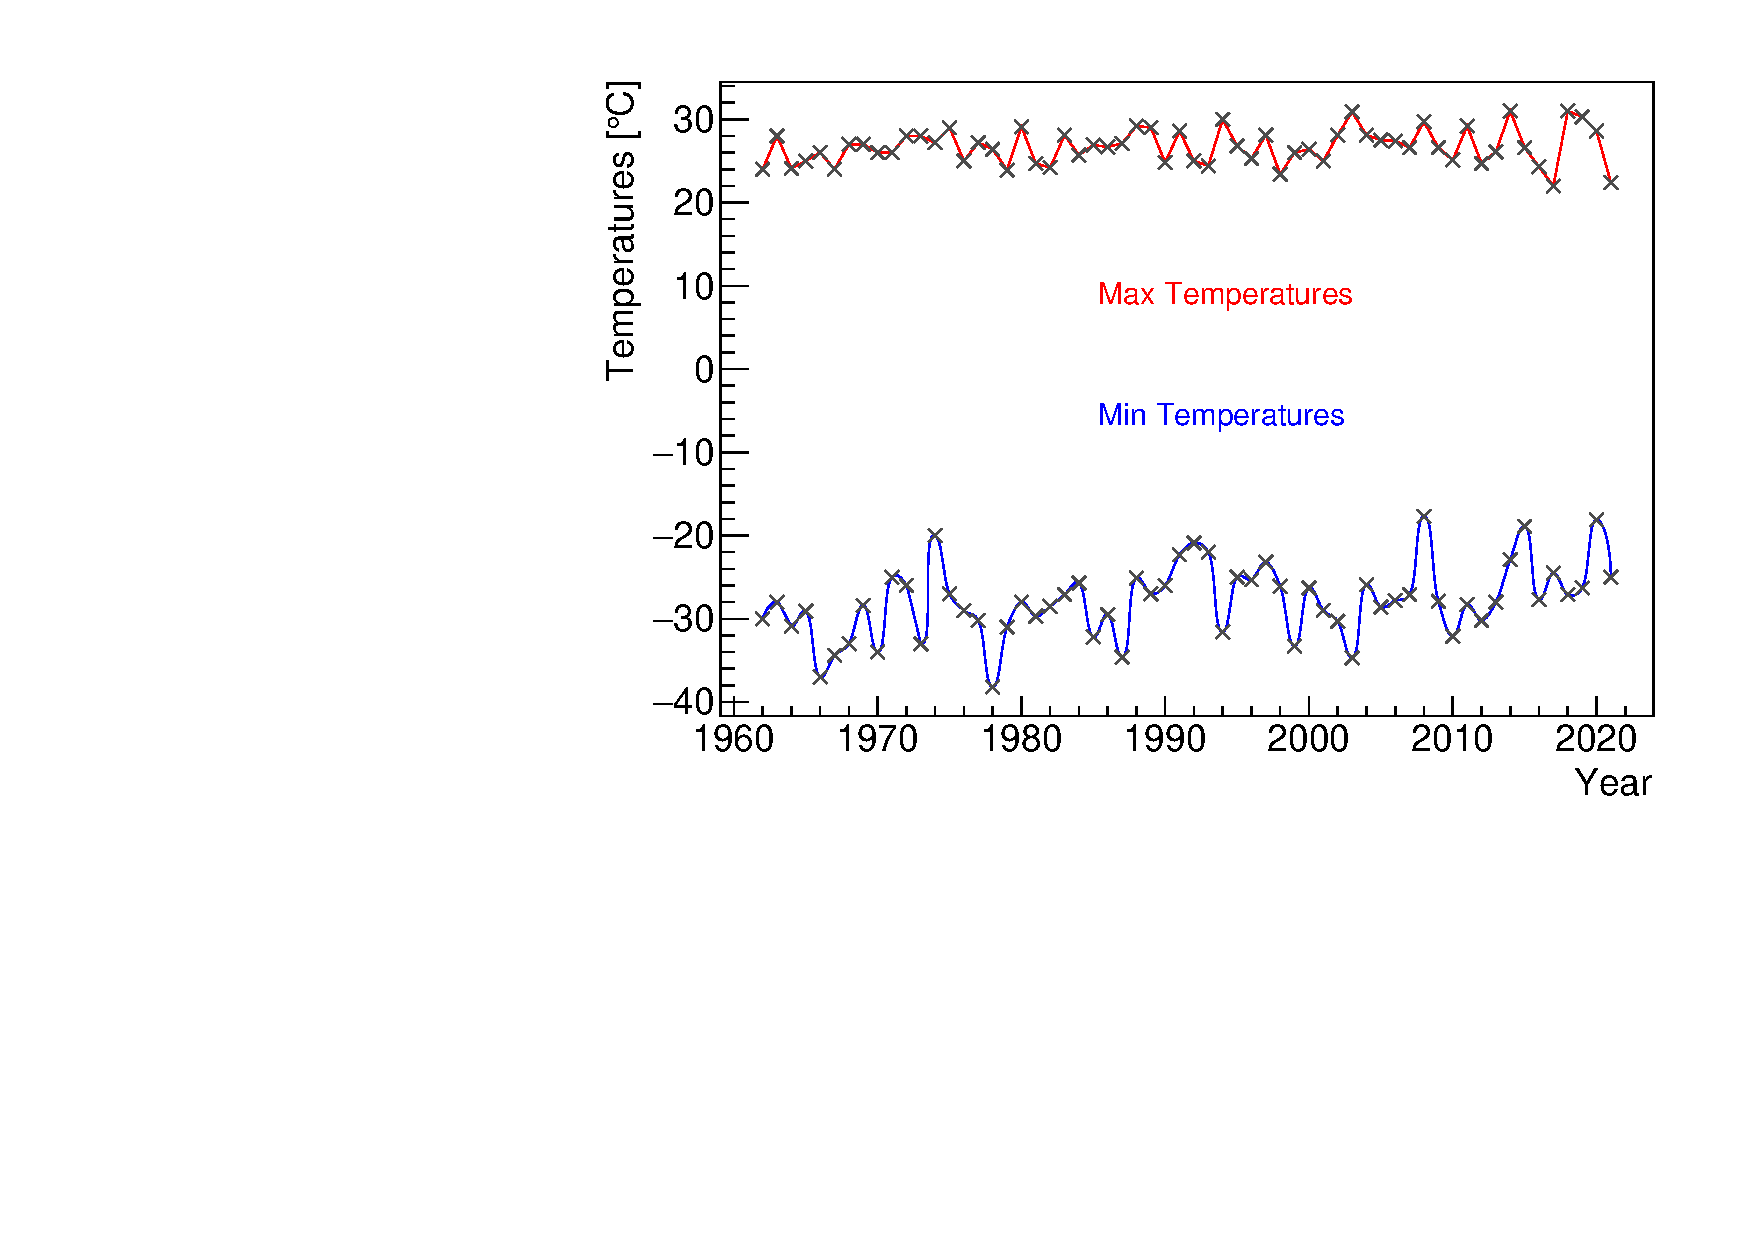
\includegraphics[width=0.5\linewidth]{Images/minmax_Umea.csv.pdf}}
    \caption{Plots illustrating how the maximum and minimum temperatures change throughout time in (a) Falsterbo, (b) Lund, (c) Borås and (d) Umeå.}
    \label{fig:MinMaxTemp}
\end{figure}
As can be seen in the figures above, both the maximum and minimum temperatures fluctuate over time. Furthermore, between adjacent years, the minimum temperature oscillates more. In general, for all the cities, the hottest days reach a temperature of 20-30$^{\circ}$C, whereas the coldest temperature drops as we go more in the North of Sweden; Falsterbo and Lund reach a minimum of -20$^{\circ}$C, while Umeås temperature drops to -40$^{\circ}$C.
\newline
\newline
Also, at the plot for Lund, one can notice a spike in the Max temperature. This is because in that particular year the temperature data recorded were less than usual, which gave us less information.



\subsection{Average daily temperature and season length}
The following figures in this section all correspond to weather data gathered from Lund and Umeå, these two cities are here chosen to showcase the results as they represent different parts of Sweden, where Lund is located in southern Sweden and Umeå is located in northern Sweden. By then plotting the average daily temperature in Lund and Umeå through time, the following plots were obtained.
\begin{figure}[H]
    \centering
    \subfloat[Lund]{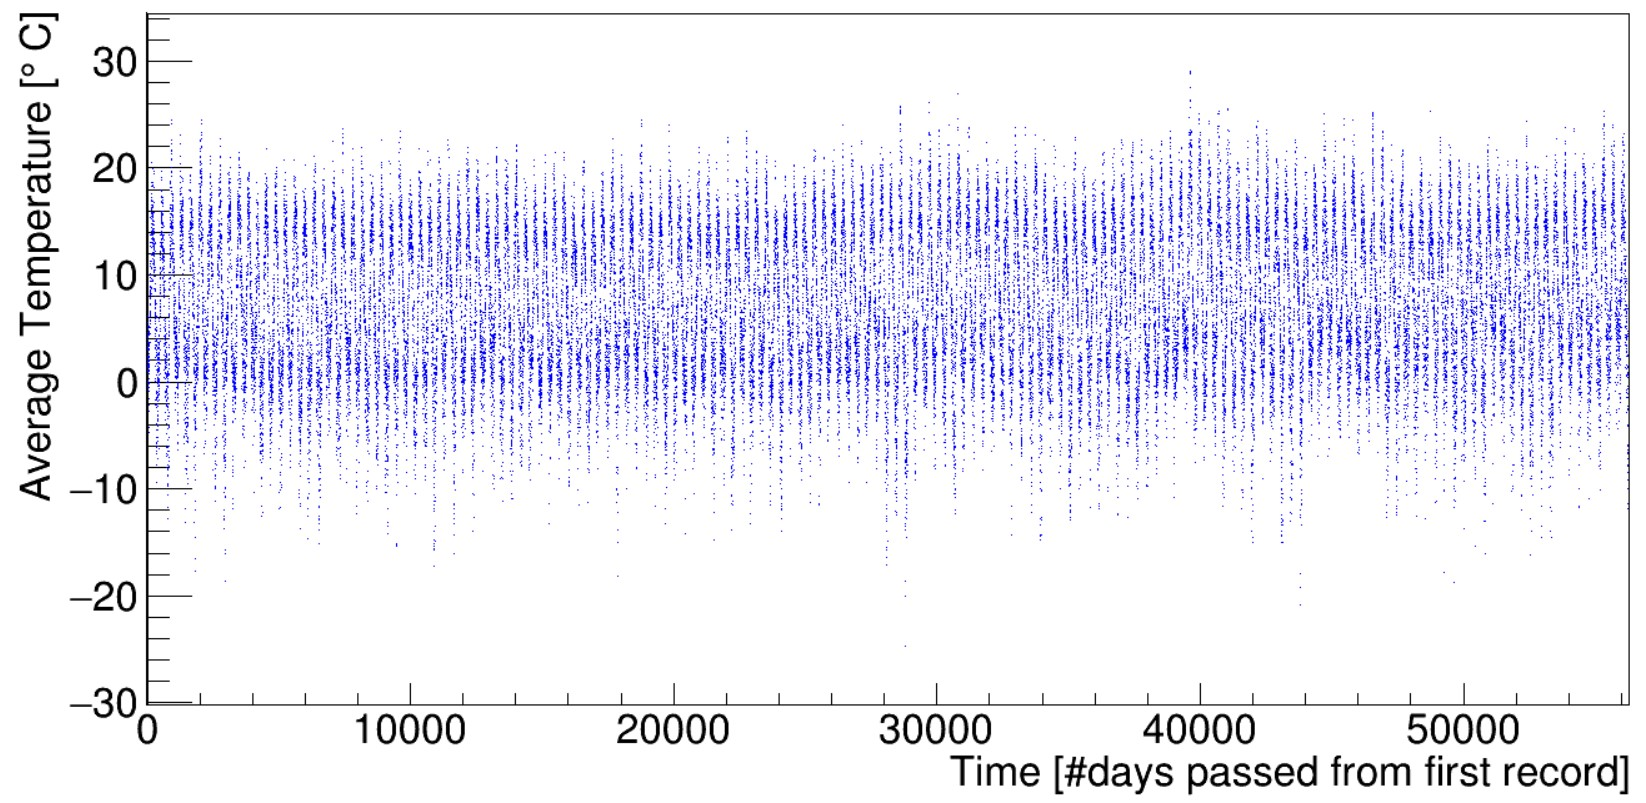
\includegraphics[width=\linewidth]{Images/Lund-daily2.png}}
    \quad
    \subfloat[Umeå]{\includegraphics[width=\linewidth]{Images/Umeå-daily.png}}
    \caption{Plots illustrating how the average daily temperature changes throughout time in (a) Lund, and (b) Umeå.}
    \label{fig:Daily_temp}
\end{figure}
From the plots in Figure~\ref{fig:Daily_temp} it is observed that there seems to be a rather continuous oscillation around a certain temperature for both cities. However, to observe the behavior closer, consider the zoomed-in versions below.
\begin{figure}[H]
    \centering
    \subfloat[Lund]{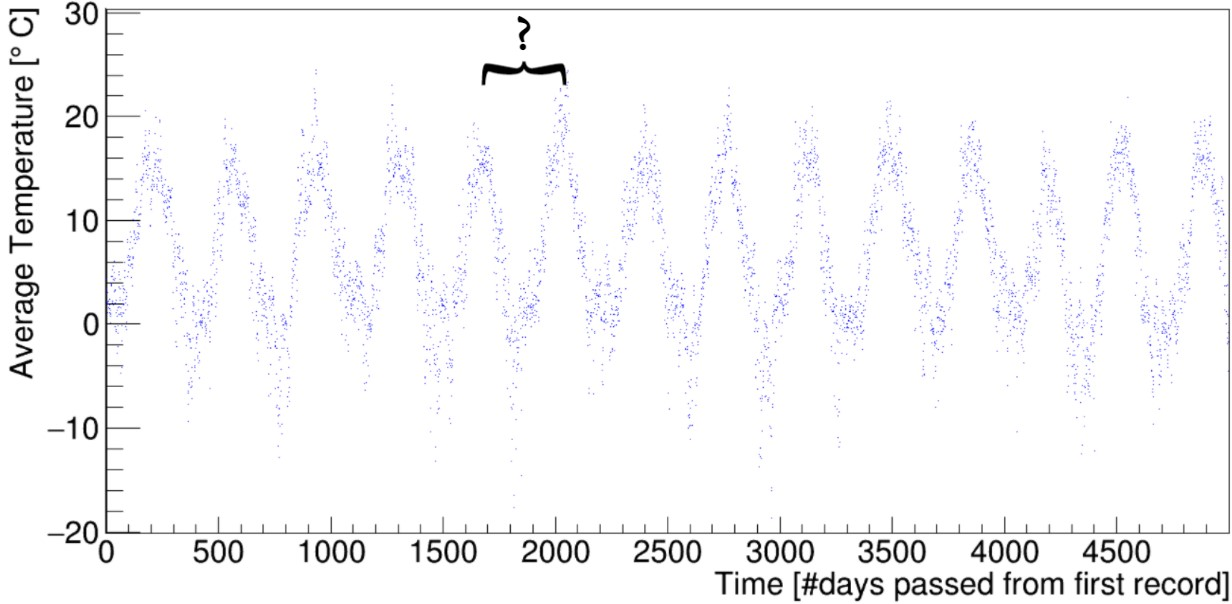
\includegraphics[width=\linewidth]{Images/Lund-daily-zoom.jpg}}
    \quad
    \subfloat[Umeå]{\includegraphics[width=\linewidth]{Images/Umeå-daily-zoom.jpg}}
    \caption{These plots show how the average daily temperature changes throughout the first 5000 days of recorded temperature measurements in (a) Lund, where "?", marks the season length (i.e. time from warmest day of a year to another), and (b) Umeå.}
    \label{fig:Daily_temp_zoomed}
\end{figure}
By considering the results seen in Figure~\ref{fig:Daily_temp_zoomed}, it is apparent that the average daily temperature is changing with a sinusoidal behavior in both of the considered cities. 

To answer the question whether the length of the seasons are changing or not, the distance (i.e. number of days) between each maximum in the plots from Figure~\ref{fig:Daily_temp} are considered. The results are seen below.
\begin{figure}[H]
    \centering
    \subfloat[Lund]{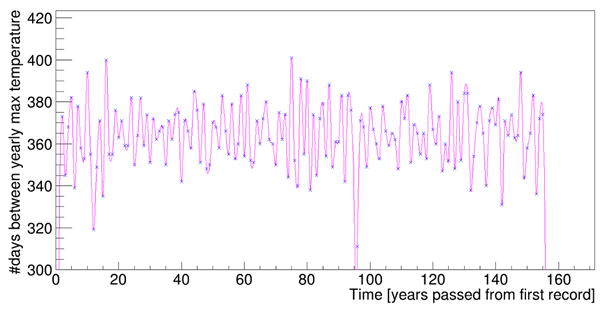
\includegraphics[width=.9\linewidth]{Images/Lund-season-length.png}}
    \quad
    \subfloat[Umeå]{\includegraphics[width=.9\linewidth]{Images/Umeå-season-length.png}}
    \caption{The plots displays how many days that passes between each yearly maximum temperature in (a) Lund, and (b) Umeå.}
    \label{fig:season_length}
\end{figure}

Note that Figures \ref{fig:Daily_temp}-\ref{fig:season_length} all correspond to weather data collected in Lund and Umeå, however, similar behavior as seen in these figures was also observed in all of the investigated data sets.


\section{Conclusions \& Outlook}
In conclusion, the analysis of the temperature data recorded by SMHI can give many insights into how the weather and climate conditions have been changing over the last one or two centuries.
\newline
In the first task, the histogram of the temperature of a single day shows that the distribution acts like a Gaussian. The mean  temperatures change with seasons and also the temperatures drop slightly as one goes more north. It is difficult to evaluate the exact nature for the northern most cities due lack to enough data.
\newline
In addition, regarding the maximum and minimum temperatures, one can see that there is a general trend of the temperature fluctuating over time. As a team, we wanted to investigate and inspect if the maximum temperature will rise over time, giving a insight of global warming. Looking closer to the graphs, one can see that the temperatures slightly rises over time for Falsterbo city and Umeå. However, one knows that for some years there is inadequate data, hence an absolute conclusion cannot be taken.
\newline
Lastly, the results in the third task show that the number of days in a season tend to fluctuate around 365 days. This suggests that the definition of a year lasting for 365 days, is valid and in accordance with the length of the seasons. In fact, when we experience the hottest day of the summer, we can conclude that on average we should expect to wait 365 days until we experience the warmest day of the next summer.
\newline
For further analysis, one could try to fit the oscillations that are seen as the passage of time where each oscillation indicates a season. From the fit, more conclusions about the season, the spread of temperatures, insights of global warming and climate change could be deduced. 



\end{document}
